\documentclass[10pt, twocolumn]{article}
\usepackage[utf8]{inputenc}
\usepackage[english]{babel}
\usepackage[T1]{fontenc,url}
\usepackage{parskip}
\usepackage{lmodern}
\usepackage{microtype}
\usepackage{verbatim}
\usepackage{amsmath, amssymb,amsthm}
\usepackage{mathtools}
\usepackage{bm}
\usepackage{tikz}
\usepackage{outlines}
\usepackage{physics}
\usepackage{algorithm}
\usepackage{algpseudocode}
\usepackage{listings}
\usepackage{enumerate}
\usepackage{float}
%\usepackage{epsfig,floatflt}
\usepackage{epigraph}
\usepackage{todonotes}
\usepackage[toc,page]{appendix}
\usepackage{enumitem}
\usepackage{multicol}
\usepackage{abstract}
\usepackage{tabularx}
\usepackage[vmargin=1.7cm, hmargin=0.7cm]{geometry}
\usepackage[margin=10pt, textfont={small, it}, labelfont={bf}, labelsep=endash]{caption}
\setlength{\columnsep}{0.5cm}
\usepackage{lipsum}

% Float page fractions
\addtolength{\dbltextfloatsep}{-0.2in}
\newcolumntype{L}[1]{>{\raggedright\arraybackslash}p{#1}}
\newcolumntype{C}[1]{>{\centering\arraybackslash}p{#1}}
\newcolumntype{R}[1]{>{\raggedleft\arraybackslash}p{#1}}

% Header/footer
\usepackage{fancyhdr}
\pagestyle{fancy}
\renewcommand{\headrulewidth}{0pt}
\usepackage[stable]{footmisc}
\rhead{}

% Fig stuff
\usepackage{caption}
\usepackage{graphicx}% Include figure files, captions for subfigures
\usepackage[margin=15pt]{subcaption}

% Referencing
\usepackage{natbib}
\bibliographystyle{dinat}
%\usepackage{varioref}
\usepackage{hyperref}
\usepackage{cleveref}

%%%% User made commands
\renewcommand{\b}{\boldsymbol}

% Expectation value E with brackets
\providecommand{\forv}[1]
{
\ensuremath{\mathbb{E}\left[#1\right]}
}
% Expectation value expressed as sum
\providecommand{\forvsum}[1]
{
\ensuremath{\frac{1}{n}\sum_{i=0}^{n-1} #1}
}
% bold math with tilde!
\providecommand{\bmt}[1]
{
\ensuremath{\bm{\tilde{#1}}}
}



\begin{document}

\newgeometry{left=2.5cm, bottom=0.7cm}
\title{FYS-STK4155 -- Project 2\\ Neural Networks and Logistic Regression}
\author{
	\begin{tabular}{rl}
        Julie Thingwall & (\texttt{juliethi})\\
        Jonas Gahr Sturtzel Lunde & (\texttt{jonassl})\\
        Jakob Borg & (\texttt{jakobbor}) \\
        \tiny{also known as the three Js of the apocalypse}
	\end{tabular}
    }
\date{}

\setlength{\epigraphwidth}{0.75\textwidth}
\renewcommand{\epigraphflush}{center}
\renewcommand{\beforeepigraphskip}{30pt}
\renewcommand{\afterepigraphskip}{50pt}
\renewcommand{\epigraphsize}{\normalsize}


\twocolumn[
\begin{@twocolumnfalse}
    \maketitle
    \epigraph{Duh - duh - duh ... duh-duh .... duhduh}
	{\textit{- Mortens Phone}}

    \begin{abstract}
    \vspace{0.5cm}
    The steady rise in computational power over the last handful of decades has given rise to a large interest in more power hungry machine learning models, like neural networks, to rival more conventional methods. In this report, we study the performance of neural networks in both regression and classification problems, and compare it to the performance of the more traditional methods of OLS regression, Ridge regression, and logistic regression. A large focus was put on the inner workings of the neural network and logistic regression models, which we both built from scratch, in Python. We have gathered, cleaned and studied data from the World Happiness Report for the regression fit, and credit card default data from a Taiwanese bank for the classification case. Hyperparameter optimization was performed over relevant parameters for all models. The neural network obtained an optimal R2 score of 0.765 in the regression case. This put it slightly behind that of Ridge, at 0.782, but head of OLS, at 0.743. In the classification case our neural network achieved an area score of 0.670, slightly tailing logistic regression, at 0.684. We also found that the classification data strongly favored a deep network, with few nodes but several layers, while the regression data seemed to prefer more narrow networks, with fewer layers, but many nodes.
\end{abstract}
\end{@twocolumnfalse}
]

\vfill

\pagebreak

\restoregeometry

\onecolumn
\tableofcontents
\twocolumn
\pagebreak

%\begin{multicols}{2}
% ██╗███╗   ██╗████████╗██████╗  ██████╗ 
% ██║████╗  ██║╚══██╔══╝██╔══██╗██╔═══██╗
% ██║██╔██╗ ██║   ██║   ██████╔╝██║   ██║
% ██║██║╚██╗██║   ██║   ██╔══██╗██║   ██║
% ██║██║ ╚████║   ██║   ██║  ██║╚██████╔╝
% ╚═╝╚═╝  ╚═══╝   ╚═╝   ╚═╝  ╚═╝ ╚═════╝
\section{Introduction}
Classification and regression are the two most common problems in machine learning, both aiming to tackle the challenge of predicting one or more properties of a data set, given some explanatory variables. While regression aims to predict some continuous quantity, classifications strives to place data points in a series of discrete categories. Both problems have for ages been rigorously studied, and approached by regression and other classical statistical methods. In recent years, the rising popularity of neural networks have brought new approaches to both problems, and, in some cases, vastly improves upon the more old school approaches.

In this report we study both classification and regression using both the more orthodox methods, and developing neural networks for both cases. In the case of classification, we build a classifying neural network and write a code for logistic regression. These two methods are both explored separately, and also compared to study the differences in performance. Likewise for regression, we build a neural network, which is bench marked against the more orthodox method of linear regression, specifically Ridge regression, where we utilize the already implemented methods found in the Python package \texttt{scikit-learn}. We will also compare the performance of our self made neural network with the Python package \texttt{Keras}. The performance, properties, pros, and cons of each method is studied by applying them to two chosen datasets. For the regression problem, we use data from the World Happiness Report, 2015-2017, trying to predict the happiness score of given countries over the period. For the classification problem, credit card default data from customers of a Taiwan bank, April-September 2005, is used, in an attempt to classify who defaults on their debt.

% ████████╗██╗  ██╗███████╗ ██████╗ ██████╗ ██╗   ██╗
% ╚══██╔══╝██║  ██║██╔════╝██╔═══██╗██╔══██╗╚██╗ ██╔╝
%    ██║   ███████║█████╗  ██║   ██║██████╔╝ ╚████╔╝ 
%    ██║   ██╔══██║██╔══╝  ██║   ██║██╔══██╗  ╚██╔╝  
%    ██║   ██║  ██║███████╗╚██████╔╝██║  ██║   ██║   
%    ╚═╝   ╚═╝  ╚═╝╚══════╝ ╚═════╝ ╚═╝  ╚═╝   ╚═╝  
\section{Theory}
\label{sec:Theory}
\subsection{Neural Networks}
\label{subsec:Theory/NN}

\subsubsection{Brief Introduction to Artificial Neural Networks}
\label{subsec:Theory/ANN_intro}
In a superficial form, artificial neural networks are computational networks of artificial neurons able to learn by an iterative process of considering training data and matching the data features with expected outputs.

Theses networks, or systems, are heavily inspired by the biological decision making network of neurons present in the human brain. A vast connected network of neurons influencing each other by sending electromagnetic signals in between them. This system is responsible for all our rational (and irrational) thinking. For example when we observe some sort of event happening around us; the information obtained is fed into our network of neurons in the brain, which weighs up our thoughts and possible responses based on the event and our prior experiences, eventually leading to some sort of decision or sensation as a result of our observations.

In artificial neural networks this behavior is mimicked in a simplified form. Layers of artificial neurons are connected together and the electromagnetic signals are replaced by mathematical functions. Each connection between neurons are represented by a weight, which acts similarly to the prior knowledge or experiences of a person, and are used to quantify the significance of each connection. The goal of a neural network is to tune these weights of every connection in order to correctly estimate some reaction, or output, given a set of inputs. There are many kinds and families of neural networks, in this report we implement one of the simplest types; a fully connected feed-forward neural network (FFNN) with backward propagation and stochastic gradient decent.

\subsubsection{Basic Expressions and Quantities}\label{subsubsec:theory_NN_basicexpressions}
\def\layersep{2.5cm}
\begin{figure}
    \centering
    
    \begin{tikzpicture}[shorten >=1pt,->,draw=black!50, node distance=\layersep]
    \tikzstyle{every pin edge}=[<-,shorten <=1pt]
    \tikzstyle{neuron}=[circle,fill=black!25,minimum size=17pt,inner sep=0pt]
    \tikzstyle{input neuron}=[neuron, fill=green!50];
    \tikzstyle{output neuron}=[neuron, fill=red!50];
    \tikzstyle{hidden neuron}=[neuron, fill=blue!50];
    \tikzstyle{annot} = [text width=4em, text centered]

    % Draw the input layer nodes
    \foreach \name / \y in {1,...,4}
    % This is the same as writing \foreach \name / \y in {1/1,2/2,3/3,4/4}
        \node[input neuron, pin=left:Input \#\y] (I-\name) at (0,-\y) {};

    % Draw the hidden layer nodes
    \foreach \name / \y in {1,...,5}
        \path[yshift=0.5cm]
            node[hidden neuron] (H-\name) at (\layersep,-\y cm) {};

    % Draw the output layer node
    \node[output neuron,pin={[pin edge={->}]right:Output}, right of=H-3] (O) {};

    % Connect every node in the input layer with every node in the
    % hidden layer.
    \foreach \source in {1,...,4}
        \foreach \dest in {1,...,5}
            \path (I-\source) edge (H-\dest);

    % Connect every node in the hidden layer with the output layer
    \foreach \source in {1,...,5}
        \path (H-\source) edge (O);

    % Annotate the layers
    \node[annot,above of=H-1, node distance=1cm] (hl) {Hidden layer};
    \node[annot,left of=hl] {Input layer};
    \node[annot,right of=hl] {Output layer};
    \end{tikzpicture}
    
    \caption{Conceptual sketch of the connections in a neural network with one hidden layer \citep{tikz_NN}. Each neuron in the preceding layers are connected to each neuron in the following layer with a weight and a bias parameter.}
    \label{fig:tikz_NN}
\end{figure}

Let's describe the basic theory in terms of a simple example network, with an input layer, one hidden layer with $m$ neurons and an output layer. Assuming a classification problem with binary outcome and a data set with a single feature; the input layer will then consist of one neuron for each data point in the data set $\bm{x} = \left(x_1,x_2,\ldots, x_n\right)$, and the output layer will have two neurons, one for each class. Each of the neurons in the input layer sends its output, which is just the data points, to each neuron in the hidden layer. The output of a layer we call $\bm{a}^l$ where $l$ indicate the layer number. In the connection between the input layer, $l=0$, and the hidden layer, $l=1$, we multiple each output with its corresponding weight variable, and add a small bias term to prevent zero values. The result is the so called weighted input which is used as input to each neuron in the hidden layer
\begin{equation}
    z_j^l = \sum_{i=1}^n w_{ji}^l a^{l-1}_i + b_j^l \qfor i\in \left[1,2,\ldots,m\right]
    \label{eq:weighted_input}
\end{equation}
with $l=1$ for the weighted input in the hidden layer. This is how the neurons communicate, the output from the previous layer $\bm{a}^{l-1}$ is used together with the corresponding weights and biases to produce the input to the next layer. The input is then handled with an activation function in each following layer, so that the output from layer $l$ is
\begin{equation}
    a_j^l = \sigma\left(z_j^l\right) = \sigma \left(\sum_{i=1}^n w_{ji}^l a^{l-1}_i + b_j^l\right)
    \label{eq:activation}
\end{equation}
where $\sigma$ is the activation function.

The activation function is the mathematical way of mimicking the way the biological neurons behave, which can be thought of as a neuron either responding or not responding (firing or not firing) based on the input. The choice of which activation function to use is just one of the many choices for hyperparameters one has to make when creating a neural network. Some of the most popular choices is the hyperbolic tangent, the Rectified linear unit (RELU) and the sigmoid function. The latter may be expressed as
\begin{equation}
    \sigma(z) = \frac{1}{1+\exp(-z)}.
    \label{eq:zigmoid_func}
\end{equation}
This function takes the value zero for large negative values of the weighted input, and the value one for large positive $z$, this we interpret as the neuron not firing or firing. The reason the sigmoid function is often used is because of its smooth behavior near $z=0$, where it goes from $\sigma = 0$ to $\sigma =1$ in a well behaved way. As we will see later this is crucial for how the network will learn, where we can infer a small change in the weights and biases in a specific layer which then produces a slightly different output from that layer. In our binary example we can define the resulting output class from the input depending on the value of the activation function in the last layer. For $\sigma(z^L) \geq 0.5$ we can define the output as class type $0$, and for $\sigma(z^L) < 0.5$ the output is class type $1$. Note that we use $l=L$ to indicate the last layer, the output layer.

The popular and simpler linear activation function, the RELU function, is expressed
\begin{equation}
    \sigma(z) =
    \begin{cases}
    & 0 \qfor z<0
    \\
    & z\qfor z\geq 0.% \qq{else}%
    \end{cases}
    \label{eq:RELU_func}
\end{equation}
This behaves quite differently than the sigmoid function, with no upper limit on the value it can take, but the same lower value, and the discontinuous behavior near $z=0$. Both functions has strengths and weaknesses, and its not perfectly clear why one seems to work better than the other in different cases. Both functions have simple derivatives, which will be important in the learning process discussed in \cref{subsubsec:Theory/NN/Backward_prop_algo}.


As mentioned, the choice of activation function is important when creating a neural network. There are a few constraints on this choice in order for the neural network to fulfill the universal approximation theorem which briefly states; a feed forward neural network with one hidden layer with a finite number of neurons are able to approximate any multidimensional continuous function on compact subsets of real functions to arbitrary accuracy given appropriate parameters and hyperparameters, \textit{if} the activation functions in the hidden layers are

\begin{multicols}{2}
\begin{itemize}
    \item bounded
    \item non-constant
    \item differentiable
    \item monotonically-increasing
\end{itemize}
\end{multicols}

This is a really powerful theorem, which gives the feed forward neural networks the potential of being so called universal approximators.

\subsubsection{Feed Forward}
\label{subsubsec:Theory/NN/FFNN}
This is the first part of the neural network, and is the method for moving information through the network from the input layer to the output layer. This step involves iterating through the layers, applying \cref{eq:weighted_input,eq:activation} in between each layer. Note that this system is easily extended to networks with more than one hidden layer. One would just keep iterating from the input layer through each hidden layer using the same equations, while changing the dimensions of the sums and vectors to reflect the number of neurons in the preceding and current layer. That is changing the $m$ and $n$ in the appropriate equations.

\subsubsection{The Cost Function}
\label{subsubsec:Theory/NN/Cost_func}
After one complete feed forward procedure, the next step is to quantify the predicting power of the neural network. This is done using a cost function, which describes how well the network has approximated the output, $\bm{a}^L$, to the desired output (or target), $\bm{t}$. Again one are free to choose any cost function, but there are a few properties which are beneficial. The unknowns variables in the \cref{eq:weighted_input,eq:activation} are the weights and biases, and ultimately these are the variables we want the network to optimize in order to predict the output correctly. As a result, it's preferred that the cost function is a smooth function with nice derivatives with respect to the weights and biases. We'll come back to this in \cref{subsubsec:Theory/NN/Gradient_descent}. Some often used cost functions, which we will stick to in this report, are the mean square error for regression problems and the cross-entropy for classification problems. These are respectively, using $\hat{\theta}$ as a short hand for the appropriate parameters for the specific problem,
\begin{gather}
    \mathcal{C}\left(\hat{\theta}\right) = \frac{1}{2n_{\rm{output}}}\sum_{i=1}^{n_{\rm{output}}} \left(a^L_i-t_i\right)^2 
    \label{eq:MSE_costfunc}
    \\
    \mathcal{C}\left(\hat{\theta}\right) = - \sum_{i=1}^{n_{\rm{output}}} \left[a^L_i\log(p(a^L_i=1)) + (1-a^L_i)\log(1-p(a^L_i=1)) \right]
    \label{eq:cross_entropy}
\end{gather}
where the $p(a^L_i=1)$ is the probability of input $x_i$ being in class $1$, and $1-p(a^L_i=1)$ is the probability of class $0$, for a binary case. In the binary example, we can interpret the sigmoid function as a probability because it ranges from zero to one. But for a more generalized case, we introduce the softmax function as the activation function used in the output layer
\begin{equation}
    a_j^L = P\left(\rm{class}\, j \,|\, z_j^L\right) = \frac{\exp(z_j^L)}{\sum_{c=0}^{C-1} \exp(z_c^L)}
    \label{eq:softmax_output}
\end{equation}
where $C$ is the total number of categories, or classes or neurons, in the final layer, and the components of $\bm{z}^L$ is the probability of the output being in each available category. Here the so called one-hot encoding is used. For our binary example the targets are defined as
\begin{equation*}
    \bm{t} =
        \begin{cases}
        &\left(1,0\right) \qfor t = 0
        \\
        &\left(0,1\right) \qfor t=1
        \end{cases}
\end{equation*}
which is compared to the output of the last layer $\bm{a}^L$, where each neuron holds the probability of the input being in each category. This is also easily extended to problems with arbitrary number of categories. To abbreviate the notation for the cross-entropy the loss function is used, so we can rewrite \cref{eq:cross_entropy} into
\begin{equation}
    \mathcal{C}\left(\hat{\theta}\right) = \sum_{i=1}^{C} \mathcal{L}_i\left(\hat{\theta}\right).
    \label{eq:cross_entropy_as_loss_func}
\end{equation}

\subsubsection{Stochastic Gradient Decent}
\label{subsubsec:Theory/NN/Gradient_descent}
With the feed forward step and cost function defined now remains the optimizing (or learning) of the network. This process center around minimizing the cost function, and for this a stochastic gradient decent algorithm is used. Here the essence of the algorithm is stated briefly, for an excellent and detailed explanation we refer to \cite{NN_deePlearning_michael}. As mentioned minimizing the cost function is really finding the optimal weights and biases for the network to correctly predict the output. After one feed forward pass the gradient of the cost function with respect to the parameters can be used to adjust the value of the weights and biases in the direction which minimizes the cost function. This is an iterative process which slightly adjust the parameters for each iteration, until the minimum in the cost function is reached. This has to be done for each weight and bias in all the layers of the network according to
\begin{align}
    w_{ji}^l &= w_{ji}^l - \eta \pdv{\mathcal{C}}{w_{ji}^l}
    \label{eq:update_weights}
    \\
    b_j^l &= b_j^l - \eta \pdv{\mathcal{C}}{b_j^l}
    \label{eq:update_biases}
\end{align}
where $\eta >0$ is the learning rate hyperparameter.

In order to introduce stochasticity in the algorithm, the data set is randomly devided into subsets called minibatches, and the gradients are approximated on these minibatches instead. This reduces the chance of our gradients to fall into local minima of the cost function, as well as speeding up the calculations as we don't operate on the entire data set at once. This also introduces another hyperparameter to the network, the size, $M$, of the minibatches. With $n$ original data points there will be $n/M$ number of minibatches, each set denoted $B_k$ for $k \in \left[1,2,\ldots,n/M\right]$. We then perform the gradient decent on each minibatch instead of the hole data set, iterating over the number of minibatches until the data set is exhausted. One full iteration over all the minibatches is called an epoch, which is yet another hyperparameter introduced, the number of epochs to train the network on. The gradients of the cost function is then written as
\begin{equation}
    \grad_\theta \mathcal{C}(\theta) = \sum_{i=1}^{N} \grad_\theta \mathcal{L}_i(\theta) \rightarrow \sum_{i\in B_k} \grad_\theta \mathcal{L}_i(\theta)
\end{equation}
summing over all the points in the respective minibatch $B_k$.

\subsubsection{Backward Propagation Algorithm}
\label{subsubsec:Theory/NN/Backward_prop_algo}
Now the last piece is the algorithm for calculating every required gradient of the cost function with respect to the appropriate parameters, as in \cref{eq:update_weights,eq:update_biases}. For this the backward propagation algorithm is implemented. Here the need for an appropriate choice of cost function becomes clear, the gradients with respect to the weights and biases of the cost function is obtained through applying the chain rule in a methodical way. Here the final equations are listed, for an in depth explanation we again refer to \cite{NN_deePlearning_michael}. The propagation is an iterative process to find the error of each layer, defined $\delta^l_j = \pdv{C}{z_j^l}$, starting from the output layer and iterating backwards to the first hidden layer. The error from the output layer is then defined as
\begin{equation}
    \delta^L_j = \pdv{C}{a^L_j}\sigma\prime(z_j^L)
    \label{eq:output_error}
\end{equation}
where $\sigma\prime(z_j^L)$ is the derivative of the activation function. With this quantity the error of the preceding layers are found by iterating backwards from $l=L$ to the first hidden layer $l=1$ by (note the reversed order in the indices for the weights)
\begin{equation}
    \delta^l_j = \sum_i \delta_i^{l+1} w_{ij}^{l+1}\sigma\prime(z^l_j).
    \label{eq:hidden_error}
\end{equation}
Using these defined error quantities the gradients with respect to weights and biases may be expressed
\begin{align}
    \pdv{C}{w_{ji}^l} &= a_i^{l-1} \delta_j^l
    \label{eq:gradient_w}
    \\
    \pdv{C}{b_j^l} &= \delta_j^l
    \label{eq:gradient_b}
\end{align}
for all layers $l\in[1,L]$. As mentioned when discussing the activation functions, its derivatives enter in \cref{eq:output_error,eq:hidden_error} acting as a weight to the error used in the gradients. This introduces a potential problem for the rate of learning in the network, especially when using the sigmoid activation, called the vanishing gradients problem. For large weighted inputs to the sigmoid function, $\abs{z}>>0$, its derivatives are close to zero. This results in the gradients for the weights and biases being really small, and so the network will require a lot of iterations to optimize the quantities through \cref{eq:update_weights,eq:update_biases}. The RELU function behaves in a different way, since its derivative is either $0$ or $1$, and so the vanishing gradients are less of a problem as long as not all of the weighted inputs become less than zero.

\subsection{Logistic regression}\label{subsec:theory_logreg}
As mentioned, neural networks is a relatively new approach to solving classification problems. A more classical way of approaching such problems is logistic regression. While similar in name to linear regression, logistic regression differs in that it aims to predict discrete data points, not continuous. In essence, logistic regression classifies data in different groups or classes based on a set of inputs or predictors. The simplest case is where the output is binary, for example if a person pays their credit card bill or not. 

In many ways, one can say that logistic regression is a very specific case of a neural network \textit{(or that a neural network is an extension of logistic regression)}, with no hidden layers and no backward propagation. Thus, much of the theory will be similar. 

\subsubsection{The sigmoid function}
While linear regression aims to find the best fit line through a set of data points, logistic regression tries to categorize data points. Thus, one needs a function where it's relatively straight forward to set a boundary between different classes. A much used example of such a function is the logistic function, or the sigmoid function, which takes the form
\begin{align}\label{eq:sigmoid_logreg_init}
    p(t) = \frac{1}{1+\exp(-t)}.
\end{align}

This function, as previously discussed in \cref{subsubsec:theory_NN_basicexpressions}, has the important property that it converges to $1$ and $0$ for large and small $t$ respectively, making it ideal for classifying binary cases. Notice that \cref{eq:sigmoid_logreg_init} is denoted as $p(t)$ and not $\sigma(z)$, as it was when speaking of neural networks. This is because, in the case of logistic regression, the sigmoid function represents a probability of a given output, not whether or not a neuron activates, making this notation more natural going forward. 

In general, given a case with a binary output $y_i = \{0,1\}$, a set of predictors $\bm{x}_i = [1, x_1, x_2,..,x_p]$ corresponding to output $y_i$, and a set of weights $\bm{\beta} = [\beta_0, \beta_1,...,\beta_p]$, the probabilities of either output can be expressed as 
\begin{align}\label{eq:sigmoid_logreg_prob}
    p(y_i = 1|\bm{x}_i, \bm{\beta}) &= \frac{1}{1+\exp(\bm{x}_i^T\bm{\beta})} \\
    p(y_i = 0|\bm{x}_i, \bm{\beta}) &= 1 - p(y_i = 1|\bm{x}_i, \bm{\beta}).
\end{align}


\subsubsection{Cost function}
Just as with linear regression, the final model is controlled by a cost function. Simply put, the cost function $\mathcal{C}(\bm{\beta})$ is some function of the weights $\bm{\beta}$. This function has the property that the $\beta$s corresponding to the minimum of $\mathcal{C}(\bm{\beta})$ are the $\beta$s yielding the model with least error. 

The important properties a cost function should have is thoroughly discussed in \cref{subsubsec:Theory/NN/Cost_func}, and it turns out that the same cost function used in a classification neural network can also be used in logistic regression. This cost function is the cross entropy function, as described in \cref{eq:cross_entropy}. Rewriting it with the notation used here yields 

\begin{align}\label{eq:cost_function_logreg}
    \mathcal{C}(\bm{\beta}) = &-[\bm{y}^T\log(p(y_i = 1|\bm{x}_i, \bm{\beta})) \notag\\
    &+ (1-\bm{y})^T\log(1 - p(y_i = 1|\bm{x}_i, \bm{\beta}))],
\end{align}
where $\bm{y}$ is a vector of all outputs $y_i$.

\subsubsection{Minimizing the cost function}
As described, minimizing the cost function is alpha and omega in logistic regression. There are many algorithms of varying complexity designed to do just this, and possibly the simplest one is simply called steepest descent. This is very reminiscent of the stochastic gradient descent described in \cref{subsubsec:Theory/NN/Gradient_descent}, but without the actual stochasticity. Steepest decent is an iterative algorithm where a new set of $\bm{\beta}$s is calculated using the gradient of the function one wishes to minimize. Simply put, it can be expressed as
\begin{align}\label{eq:steepest_descent}
    \bm{\beta}_{i+1} = \bm{\beta}_i - \eta\pdv{\mathcal{C}}{\bm{\beta}},
\end{align}
where $\eta > 0$ is the step size, or more commonly the learning rate of the algorithm, and the gradient $\pdv{\mathcal{C}}{\bm{\beta}}$ is expressed as

\begin{align}\label{eq:cost_function_gradient}
    \pdv{\mathcal{C}}{\bm{\beta}} = -\bm{X}^T(\bm{y}-\bm{p}),
\end{align}
where $\bm{p}$ is a vector containing the probabilities $p(y_i|,x_i,\bm{\beta})$ and $\bm{X}\in\mathbb{R}^{n\cross p}$ is the design or feature matrix holding all predictors.

\subsection{Error metrics}
\label{subsec:Method/Error_metrics}
To judge the proficiency of a model, one can employ some appropriate error metrics, making comparisons of models possible. For regression, the \textbf{R2 score} is commonly used. It is expressed as 
\begin{align}
    R2(Y,\ Y_\text{pred}) = 1 - \dfrac{MSE(Y,\ Y_\text{pred})}{MSE(Y,\ \overline{Y})}, 
\end{align}
where $Y$ is the true values of some output dataset, $\overline{Y}$ is the average of $Y$, $Y_\text{pred}$ is the predicition on $Y$. The R2 score represents 1 minus the ratio between the mean squared error of the prediction, and the mean squared error one would get from simply predicting the average of the model. In other words, R2 ranges from 0 to 1, with 0 representing the score of a completely naive model, and 1 a perfect model. The main advantage of the R2 score over mean squared error, is that it to some degree scaled by how difficult the model is to predict in the first place. It is also unitless.

For classification, two error metrics can be emoployed, among others. The first one being the \textbf{accuracy score}
\begin{align}
    \text{Accuracy} = \dfrac{\text{Nr. of correct predictions}}{\text{Total nr. of predictions}},
\end{align}
which is simply the fraction of correct predictions. While this error metric is easily interpretable, it has one main drawback: It can be very biased if the dataset is biased. As an example, given a data set where 90\% of the outputs are negatives one can get an accuracy of 90\% by simply guessing that every output is negative.

In other words, when dealing with biased datasets, a metric which doesn't carry this bias is prefered. The \textbf{area score}, or "Area Under the ROC Curve" score, is one such metric, as it takes into account biases in the dataset. The area score will typically be ~0.5 for any completely naive model, irregardless of bias in the dataset. The metric is explained in detail in \cite{TowardsDataScienceMetrics}.




% ███╗   ███╗███████╗████████╗██╗  ██╗ ██████╗ ██████╗ 
% ████╗ ████║██╔════╝╚══██╔══╝██║  ██║██╔═══██╗██╔══██╗
% ██╔████╔██║█████╗     ██║   ███████║██║   ██║██║  ██║
% ██║╚██╔╝██║██╔══╝     ██║   ██╔══██║██║   ██║██║  ██║
% ██║ ╚═╝ ██║███████╗   ██║   ██║  ██║╚██████╔╝██████╔╝
% ╚═╝     ╚═╝╚══════╝   ╚═╝   ╚═╝  ╚═╝ ╚═════╝ ╚═════╝
\section{Method}
\subsection{Data}
We gathered one dataset which presents a regression problem, and one which presents a classification problem. This sections presents both datasets, as well as the analysis and cleaning done on the data.

\subsubsection{World Happiness Report - regression case}
For the regression problem we used data from the World Happiness Report (WHR), years 2015, 2016, and 2017. The dataset was found at this link (\url{https://www.kaggle.com/unsdsn/world-happiness/}), and the data is explained and explored in depth in the World Happiness Reports themselves, found at this link (\url{https://worldhappiness.report/}).

The data presents 7 columns, explained in \cref{tab:WH}. We will attempt to predict the given happiness score given by WHR using the columns 1-6 as explanatory variables. The columns are a combinations of purely objective data (GDP and life expectancy), as well as 4 columns based on questionnaires given by the Gallup World Poll. The full description of the columns, as well as the questions employed by the Gallup World Poll, can be found in the WHR itself.


\begin{table}[H]
    \centering
    \begin{tabular}{R{0.7cm} p{3cm} p{4cm}}
    %\begin{tabular}{r r r}
    \textbf{Col.\newline Nr} & \textbf{Column\newline Description} & \textbf{Value\newline Description} \\
    \hline 
         0  & Happiness Score  &  The level of happiness, in the range 0-10, given by the World Happiness Report.\\
     \hline
         1  & Economy  &  Log GDP per Capita, using PPP (purchasing power parity).\\
    \hline
         2  & Family  &  Average response to question regarding support from family and friends, range [0,1]. \\
    \hline
         3  & Health  &  Life expectancy, scaled to range [0,1].\\
    \hline
         4  & Freedom  &  Averaged response to question about freedom in life, range [0,1]. \\
    \hline
         5  & Trust  &  Averaged response to question about level of government corruption, range [0,1].\\
    \hline
         6  & Generosity  &  Average response to question of personal generosity, range [0,1].
    \end{tabular}
    \caption{Table describing the columns of the world happiness dataset. For columns 1, 2, 4, 5, and 6, the numbers are gathered from the Gallup World Poll. Column 1 is gathered from the World Development indicators released by the World Bank, while column 3 is gathered from the World Health Organization.}
    \label{tab:WH}
\end{table}

The report contained the same columns for all three years, and we simply added the data from the different years together, such that e.g, Norway 2015 and Norway 2016 are two separate data points, with their own happiness score (and other variables).


\subsubsection{Credit card defaults - classification case}
For our classification problem, we used credit card default data (from now on refered to as the CC data) found on the UCI machine learning repository, found at this link (\url{https://archive.ics.uci.edu/ml/datasets/default+of+credit+card+clients}). The data contains 24 columns, explained in \cref{tab:CC}, and is gathered from credit card usage of 30'000 customers of a Taiwanese bank, over the span of April through September 2005.

The dataset contains information about the customers gender, educations, marital status, age, as well as their given credit cap in NT dollar (New Taiwan dollar), and information about their bills and repayments the last 6 months (April - September 2005). With all of these as explanatory variables, we will attempt to classify the final column of the set, which says whether the customer defaulted on their credit card debt the following month (October 2005).

\begin{table}[H]
    \centering
    \begin{tabular}{R{0.7cm} p{3cm} p{4cm}}
    %\begin{tabular}{r r r}
    \textbf{Col.\newline Nr} & \textbf{Column\newline Description} & \textbf{Value\newline Description} \\
    \hline 
        0   & Given Credit Limit & Amount of given credit, in NT dollars.\\
    \hline
        1   & Gender & {1 = male\newline 2 = female} \\
    \hline
        2   & Education & {1 = grad school \newline 2 = university \newline 3 = high school \newline 4 = other} \\
    \hline
        3   & Marital Status & {1 = Married \newline 2 = Single \newline 3 = Other} \\
    \hline
        4   & Age & Age in years.\\
    \hline
        5-10 & Repayment status for a given month. & {-1 = paid duly \newline 1 = delayed 1 month \newline ... \newline 9 = delayed 9 months}\\
    \hline
        11-16 & Bill amount for a given month. & Bill amount in NT dollar. \\
    \hline
        17-22 & Payment amount for a given month. & Payment amount in NT dollar. \\
    \hline
        23    & Defaulted on payment next month. & {1 = Yes \newline 0 = No}
    \end{tabular}
    \caption{Table describing the columns of the credit card dataset, which contains information of Taiwanese credit card customers. The columns for repayment status, bill amount, and repayment amount have 6 values, representing the months of April through September of 2005, in reverse order. The final column represents whether the individual defaulted on their payment the month of October 2005.}
    \label{tab:CC}
\end{table}



\subsubsection{Data cleaning}
\label{sec:data_cleaning}
The WHR data was found to be extremely well behaved, having values in reasonable ranges with no outlying, missing, or otherwise bad behaving values. Therefore, no additional cleaning was needed for the regression dataset, and it was used as-is.

The credit card dataset have a handful of columns that need some sort of handling. The columns 1 through 10 are all discrete, with no possibility for large outliers. They do, however, have a large amount of undefined values. Columns 5-10, containing the repayment status, are defined for values of -1, and 1-9. However, as much as 53\% and 13\% of the entries in these columns take on the values of 0 and -2, respectively. A whooping 86\% of the data contains 0 or -2 in at least one of these columns. These values are undefined by the provider of the data, but throwing away all this data would be a great sacrifice. Probably, one of these values refer to the data simply being missing or unavailable. Why there are two options for this, is unknown. We figured the value of 0 seemed appropriate for undefined values, and chose to set all values of -2 to 0 instead, while leaving the zeros be.

Columns 1-4 contain \textit{some} values of 0, which again are technically undefined, but given they number in the sub-0.1\%, we'll simply leave them be.

Columns 11 through 22, as well as 0, all contain continuous\footnote{Technically, money is discrete, but the values are so much larger than the discreteness size, making them almost continuous, for practical purposes.} values with units of NT dollars. These columns may have arbitrarily large values, and were observed to contain worrisome outliers.

We employed a common outlier removal technique, outlined in \cite{TowardsDataScienceOutlier}. It involves dividing the dataset by 3 quantiles, Q1, Q2, and Q3, which, in ascending order, splits the data in 4 chuncks of equally many points, each containing 25\% of the data. The \textit{interquartile range} (IQR), which is the range which contains the middle 50\% of the data, is defined as
\begin{align*}
    IQR = Q3 - Q1
\end{align*}
These quantities have the advantage of not being affected by outliers, since they only rely on the distribution of the data in the 0.25 - 0.75 percentile range.

It is common to remove data falling outside something like a $1.5\cdot IQR$ interval outside the first and third quantile. Because of the shape of our data\footnote{Our data is mostly very shallow on the upper range, and very steep on the lower range. The data contains amounts of money in a population, which is known to often follow a Pareto distribution, or other similarly steep curves.}, we settle on a $1.0\cdot IQR$ interval on the lower side, and a $2.0\cdot IQR$ interval on the upper side. To summarize, for outlier removal of the columns 11 - 22, and 0, we removed all values that did not fall in the range
\begin{align*}
    \big[Q1 - 1.0\cdot IQR,\ Q3 + 2.0\cdot IQR\big]
\end{align*}


\subsection{Polynomial Regression - OLS and Ridge}
To establish a baseline for our neural networks, we implemented OLS and Ridge polynomial regression, with the intention of giving an idea of what kind of performance to expect. A comprehensive walkthrough of these methods can be found in \cite{Project1}. In summary, OLS serves as a very simple polynomial regression model, while Ridge builds upon it by introducing a suppression parameter $\lambda$, which reduces its tendency to overfit.

Using the WHR data, with a held-back testing set of 10\%, we ran both OLS and Ridge for polynomial degrees 1 through 8, and Ridge with $\lambda \in [10^{-4},\ 10^2]$. The R2 score of the model applied to the testing data were averaged over 1000 runs to give consistent results. The implementation and results can be found in \texttt{world\_happiness\_linreg.ipynb}.

\subsection{Logistic Regression}
As with the regression case, we also wanted to establish a baseline for the classification neural network. To do so, we implemented logistic regression, following the theory described in \cref{subsec:theory_logreg}, with the goal to study the CC data.

Our implementation was pretty straight forward. We wrote a class \texttt{LogReg} which takes in a matrix $\bm{X}$ of all predictors, a vector $\bm{Y}$ of all outputs, number of epochs and a learning rate. The number of epochs is simply the number of iterations used in the gradient descent algorithm. 

To explore how logistic regression behaves for different parameters, we ran the code for different combinations of epochs and learning rates. Specifically with epochs in the range $100\cdot2^n$ for $n \in [0,6]$ and learning rates $10^n$ for $n\in[0,-5]$. To make sure we got reliable results, we ran each combination of parameters 40 times and calculated an average of both the accuracy- and area score. This implementation can be found in \texttt{credit\_card\_Logreg.ipynb}.


\subsection{Neural Network Design}
\label{subsubsec:Method/Building_NN}
Our goal for the neural network was to use it for both regression and classification problems, with as high adaptability as possible regarding all the hyperparameters. We therefore implemented an object oriented structure, as to not change the neural network code itself depending on the type of problem.

\subsubsection{Code Structure}
\label{subsubsec:Method/NN/code_structure}
The code consist of three modules; the main class for the neural network and two slightly different classes to use for either classification problems or regression problems\footnote{These classes can be found in \texttt{neural\_network.py}, \texttt{classification\_problem.py} and \texttt{regression\_problem.py} respectively.}.
The neural network class itself is written in a very general way, following the equations from \cref{subsec:Theory/NN} closely without specifying either the cost function or the activation functions used. These are determined in either the classification problem class or the regression class, which are used as input to the neural network, and from now on referred to as the problem classes. When initializing the problem classes the type of activation functions to be used in the hidden layers and the output layer are set, as well as what cost function to use. These classes are written in a way so that it is easy to extend the system to include any activation functions and cost functions in the future.

Also, the equations in \cref{subsec:Theory/NN} are rewritten into matrix vector multiplications to improve the performance of the calculations using the numpy library in python. Thus, for example, \cref{eq:weighted_input} and \cref{eq:hidden_error} simply becomes
\begin{align}
    \bm{z}^l &= \left(\bm{w}^l\right)^T\bm{a}^{l-1} + \bm{b}^l \label{eq:weighted_input_matrix}
    \\
    \bm{\delta}^l &= \bm{\delta}^{l+1}\left(\bm{w}^{l+1}\right)^T \odot \sigma\prime(\bm{z^l}).
\end{align}

\subsubsection{Network Architecture}
\label{subsubsec:Method/NN/architecture}
All hyperparameters, including the number of layers and the number of neurons in each of them, are set in the initialization of the network. 

\paragraph{Input and output layer} The number of neurons in the input layer are determined by the input data it self, having as many neurons as there are features in the data. The neurons in the output layer has to be set explicitly, determined by the type of problem and the data to be analyzed. For our cases, we used one-hot encoding for the binary classification problem with two neurons in the output layer. Each neuron then outputs the probability of the input being in each class. For the regression case only one output neuron where used, outputting a vector with values for each input point. Also, the activation function used in the output layer is set by the problem class, and used together with the cost function to determine to output error. Using softmax and cross-entropy for classification results in an output error of
\begin{equation}
    \bm{\delta}^L = \bm{a}^l-\bm{t}.
\end{equation}
Using the mean squared error for regression results in
\begin{equation}
    \bm{\delta}^L = \frac{1}{n_{\rm{output}}}\left(\bm{a}^l-\bm{t}\right)\odot \sigma\prime(\bm{z}^L).
\end{equation}

\paragraph{Hidden layers} The number of hidden layers and neurons in them are given as input to the network as a simple list containing the numbers of neurons to be used in each layer. Each layer only communicates with its closest neighbours so the shapes of the matrices used in the hidden layers all are determined by the number of neurons in the current and the previous layers. The activation function used in all the hidden layers are determined again by the problem class.

All the weights in the hidden and output layers are initialized with a small random value from the normal distribution with mean zero and a standard deviation of $0.05$, with appropriate shapes as discussed. The biases for each layer is simpler, as its only one bias per neuron, and its initialized to a small nonzero value of $0.01$ to remove zero inputs.

\subsubsection{Training The Network}
\label{subsubsec:Method/NN/training}
The stochastic gradient descent discussed in \cref{subsubsec:Theory/NN/Gradient_descent} are implemented as the training algorithm. The number of epochs and the size of each minibatch is taken as input when initializing the network. The gradient descent algorithm loops over the number of epochs, and the number of iterations for each epoch which is determined from the batch size and the number of data points to exhaust each epoch. For each iteration a subset of the full data is chosen at random with replacement from iteration to iteration. The network then trains on these subsets instead of the full data set, sending the subset through the feed forward pass and the backward propagation, following the discussion in \cref{subsubsec:Theory/NN/Gradient_descent,subsubsec:Theory/NN/Backward_prop_algo}. Note that there is a small difference in the way the backward propagation algorithm is implemented compared to the equations listed, which will be explained in \cref{subsubsec:Method/Implementation_backprop}. The descent method is implemented with some keyword arguments for tracking how well the network trains as a function of epochs. This tracking is a major performance hit, and so it is possible to turn off and on as needed. Again the code is implemented in a way that it is easy to specify and extend the metrics which are tracked. For regression we used the popular R2 score, and for classification the accuracy score was used, discussed in \cref{subsec:Method/Error_metrics}.

\subsubsection{Implementation of Backward Propagation}
\label{subsubsec:Method/Implementation_backprop}
In order to simplify the implementation, the backward propagation algorithm uses two loops over the layers in the network. This way we found the indexing of the arrays and lists in use to be easiest, as well as dividing the method into two parts making debugging easier. The code is primarily intended for relatively small networks, and so this is not a big performance hit.  The algorithm first find the output error according to \cref{eq:output_error}, and uses this to find the errors in all the hidden layers by \cref{eq:hidden_error} attractively. Here we utilize the negative indexing of python so that we can establish a list of errors, but where the first element is the output error and the last element is the error of the first hidden layer. Then this list is reversed, and the method loops over the layers again starting from the first hidden layer to the output layer. The gradients are found using the previously found errors and activations from the feed forward pass. Here the code differ from the theory in \cref{eq:gradient_w} because of the way each list of activations and errors are defined. As we don't have an error for the input layer, when looping through the layers the list of activations are skewed once relative to the errors. Thus the equation reads like

\begin{small}
\begin{verbatim}
for l in range(L+1):
    ...
    grad_w_list.append(np.matmul(a_list[l].T,error_list[l])
    ...
    weights_list[l] -= eta*grad_w_list[l]
\end{verbatim}
\end{small}



\subsection{Employing the Neural Network}
In addition to our own implementation, we build a neural network in Keras, which is a Python module build on top of the popular machine learning module Tensorflow. Keras offers very high level and simplistic implementations of neural networks, and we used it as a testing ground and comparison tool for our own network.

At first, we implemented an identical network structure both in our own NN class, and in Keras, to the best of our ability. Running with 2 hidden layers of 16 neurons, with the ReLu activation function, a batch size of 32, and a learning rate of 0.001, we ran both implementations, and plotted the train and test accuracy as a function of epochs. This was done both for classification, which can be found in \texttt{credit\_card\_NN\_TF.ipynb} for Keras, and in \texttt{running\_NN\_classification.py} for our own implementation, and for regression, which can be found in \texttt{world\_happiness\_NN\_TF.ipynb} for Keras, and in \texttt{running\_NN\_regression.py} for our own implementation.

Timing was also performed between the Keras implementation and our own. We ran both implementations for 1000 epochs, with a similar setup as described above, expect the size of the number of neurons per layer, which was varied between $10^1$ and $10^{3.5}$. We ran the timings 20 times and averaged them, for increased accuracy. The implementation can be found in \texttt{Timing.ipynb}.


\subsection{Hyperparameter Optimization}
\label{sec:HP_method}
As in most statistical models, we wish to tune the different hyperparameters of the model to optimal values. This involves taking every parameter that can be freely tuned, like learning rate, and trying a lot of different values. When multiple such hyperparameters are present, every combination of them should be tested, as they are often strongly correlated.

Neural networks contain a very large amount of such hyperparameters, unlike simpler methods, like logistic regression. Even in their most basic form, they often contains something like 5 or 10 hyperparameters, ranging from what types of activation functions used, to what kind of optimizer used, to number of layers. This problem presents itself both for classification and regression neural networks, and presents some problems. The first and biggest problem is the runtime of such an optimization. Ideally, we would like to run something like 10 hyperparameters, where we would like each to take on average, perhaps 5 values each. This means $5^{10} \approx 10\text{ million}$ combinations, where each configuration needs to be averaged over a large number of runs, to ensure consistent results.

The second problem is visualizing what combinations of hyperparameters give the best results. One could of course just state the best combinations of parameters, but the bigger picture is often of interest as well, especially since the performance of the parameters are often strongly correlated (tuning the learning rate often requires tuning the number of epochs, for example).

With this in mind, limited ourselves to four hyperparameters, namely number of layers, number of neurons per layer, number of epochs, and learning rate. After some initial testing, we found a reasonable range of values for each parameter. The chosen hyperparameters are listed in \cref{tab:HP_list_reg} for regression, and in \cref{tab:HP_list_clas} for classification. The total combinations number 240 and 108, respectively. Every combination was run 40 times, on a randomly selected held back 10\% test data, and the respective test score (R2 or area score) averaged over the runs. Due to time constraints, the hyperparameter optimization was performed using a neural network implemented in Keras, and not our own implementation. The implementations can be found in \texttt{world\_happiness\_NN\_TF.ipynb} for regression, and \texttt{credit\_card\_TF\_NN.ipynb} for classification.

\begin{table}[H]
    \centering
    \begin{tabular}{l l}
        \hline
        Number of layers: & $1,\ 2,\ 4$ \\
        \hline
        Neurons per Layer: & $4,\ 8,\ 16,\ 32$ \\
        \hline
        Epochs: & $200,\ 400,\ 800,\ 1600,\ 3200$ \\
        \hline
        Learning Rate: & $0.01,\ 0.001,\ 0.0001,\ 0.00001$ \\
        \hline
    \end{tabular}
    \caption{Table showing set of hyperparameters used for hyperparameter optimization of WHR regression neural network.}
    \label{tab:HP_list_reg}
\end{table}

\begin{table}[H]
    \centering
    \begin{tabular}{l l}
        \hline
        Number of layers: & $1,\ 2,\ 4$ \\
        \hline
        Neurons per Layer: & $4,\ 8,\ 16,\ 32$ \\
        \hline
        Epochs: & 50,\ 100,\ 200 \\
        \hline
        Learning Rate: & $0.01,\ 0.001,\ 0.0001$ \\
        \hline
    \end{tabular}
    \caption{Table showing set of hyperparameters used for hyperparameter optimization of CC classification neural network.}
    \label{tab:HP_list_clas}
\end{table}



% ██████╗ ███████╗███████╗██╗   ██╗██╗  ████████╗███████╗
% ██╔══██╗██╔════╝██╔════╝██║   ██║██║  ╚══██╔══╝██╔════╝
% ██████╔╝█████╗  ███████╗██║   ██║██║     ██║   ███████╗
% ██╔══██╗██╔══╝  ╚════██║██║   ██║██║     ██║   ╚════██║
% ██║  ██║███████╗███████║╚██████╔╝███████╗██║   ███████║
% ╚═╝  ╚═╝╚══════╝╚══════╝ ╚═════╝ ╚══════╝╚═╝   ╚══════╝

\section{Results}
\subsection{Data}
\subsubsection{World Happiness data}
As the WHR data was found to be of acceptable quality, it was employed unchanged, with no data cleaning performed. It contained a total of 470 data points, corresponding to over 150 countries over the span of 3 years. The distribution of values by feature is shown in \cref{fig:WH_data_hist}. We see that all features have very reasonable ranges on their data, most in the order of unity.

Figure \ref{fig:WH_corr} shows the correlation matrix of the WHR data. We observe that all our explanatory variables correlate positively with the happiness score, and most of them quite a lot, with the two best predictors seemingly being economy and health. The generosity score stands out at the only parameter without significant correlation to happiness.


\begin{figure}[H]
    \centering
    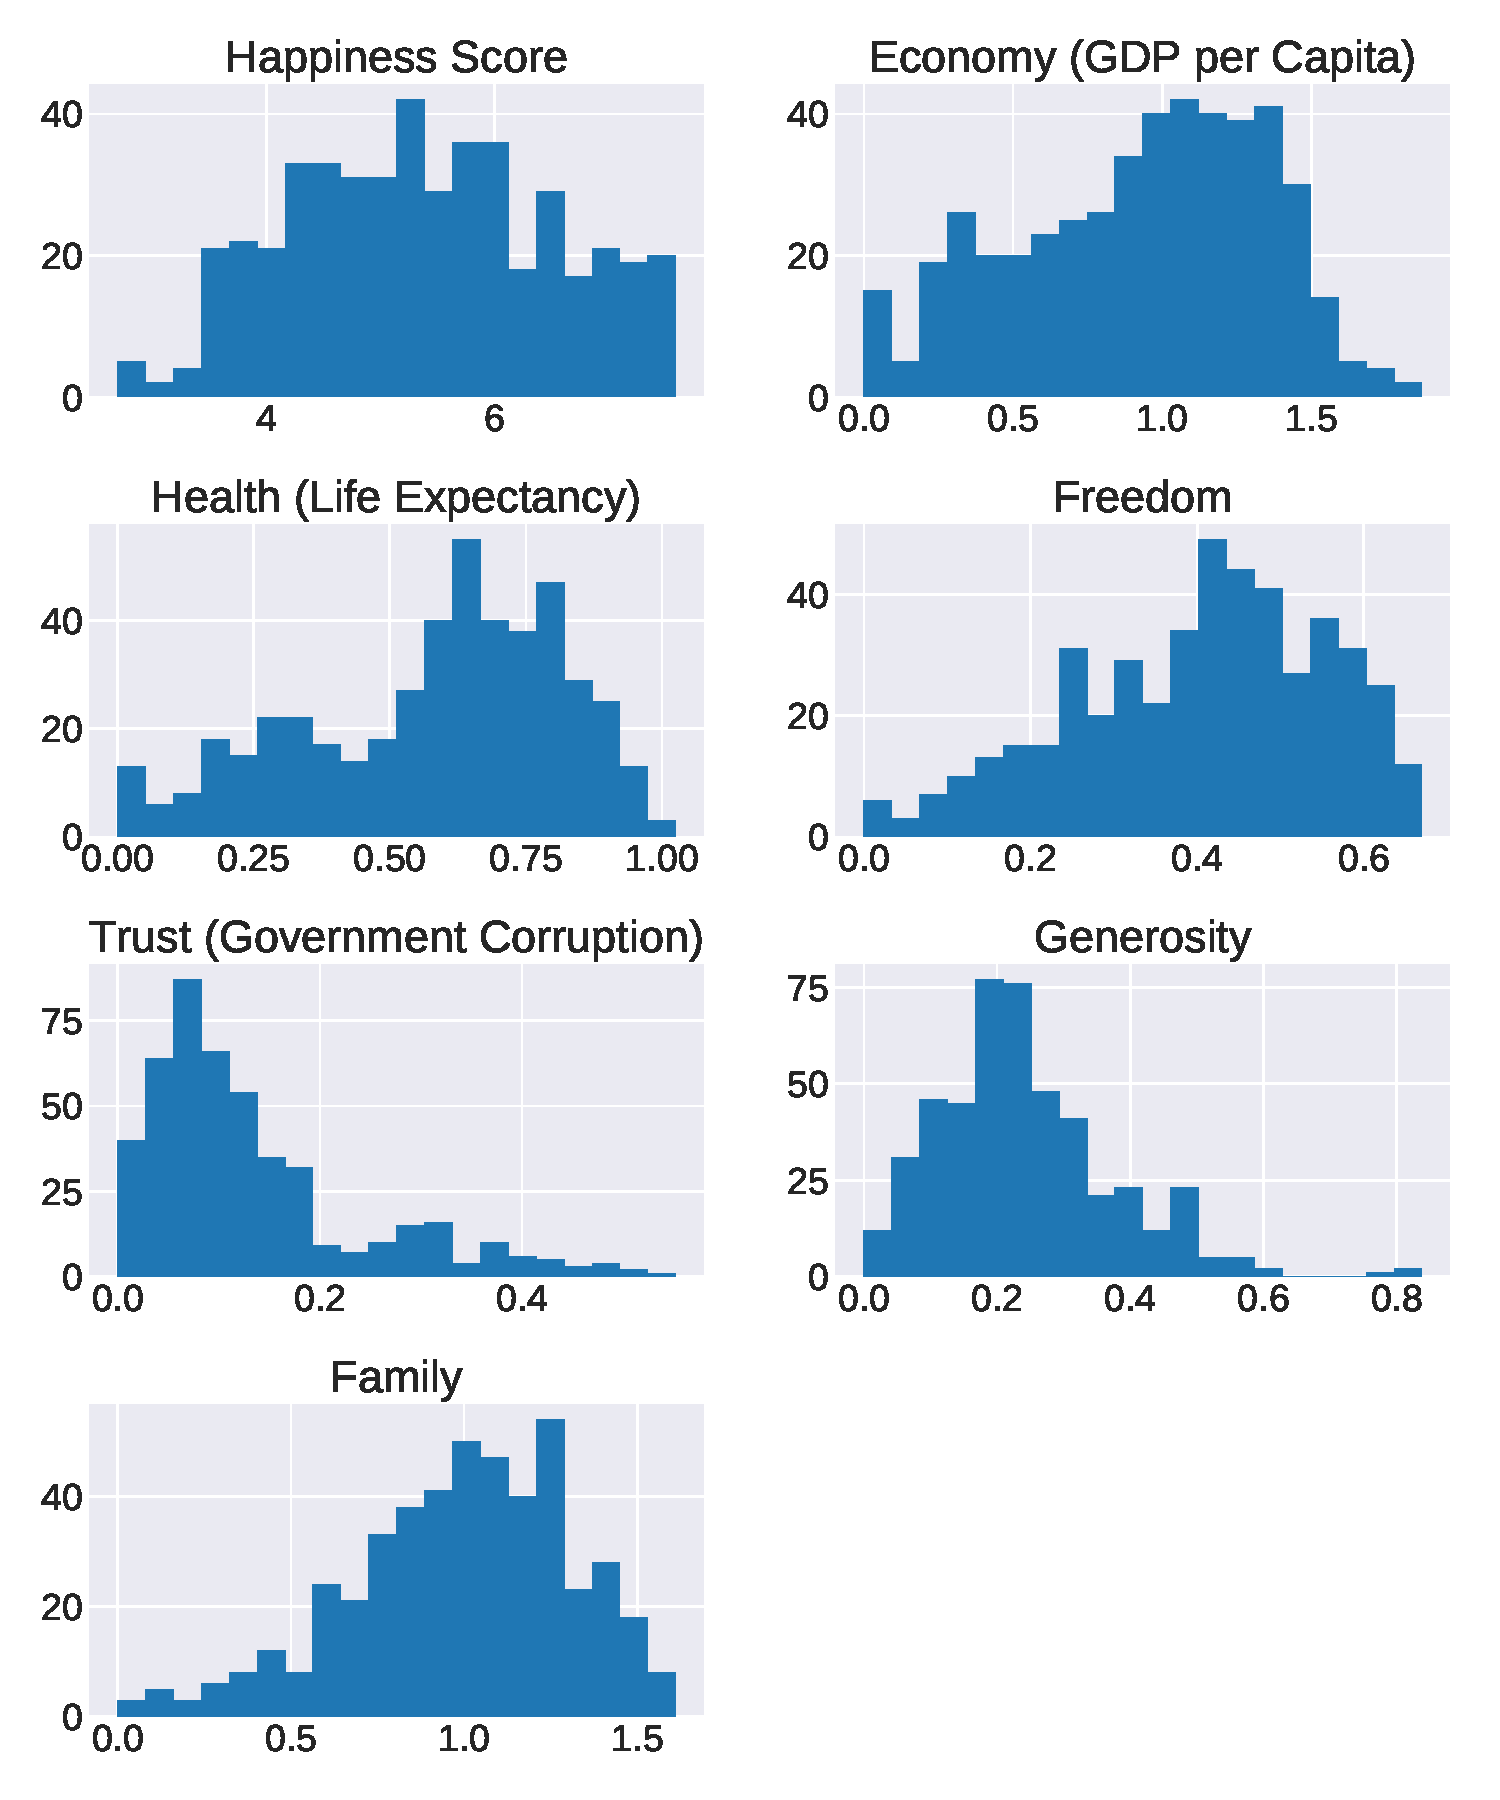
\includegraphics[scale=0.38]{../figs/WH_data_hist.pdf}
    \caption{Histogram showing the distribution of values in the WHR dataset.}
    \label{fig:WH_data_hist}
\end{figure}


\begin{figure}[h]
    \centering
    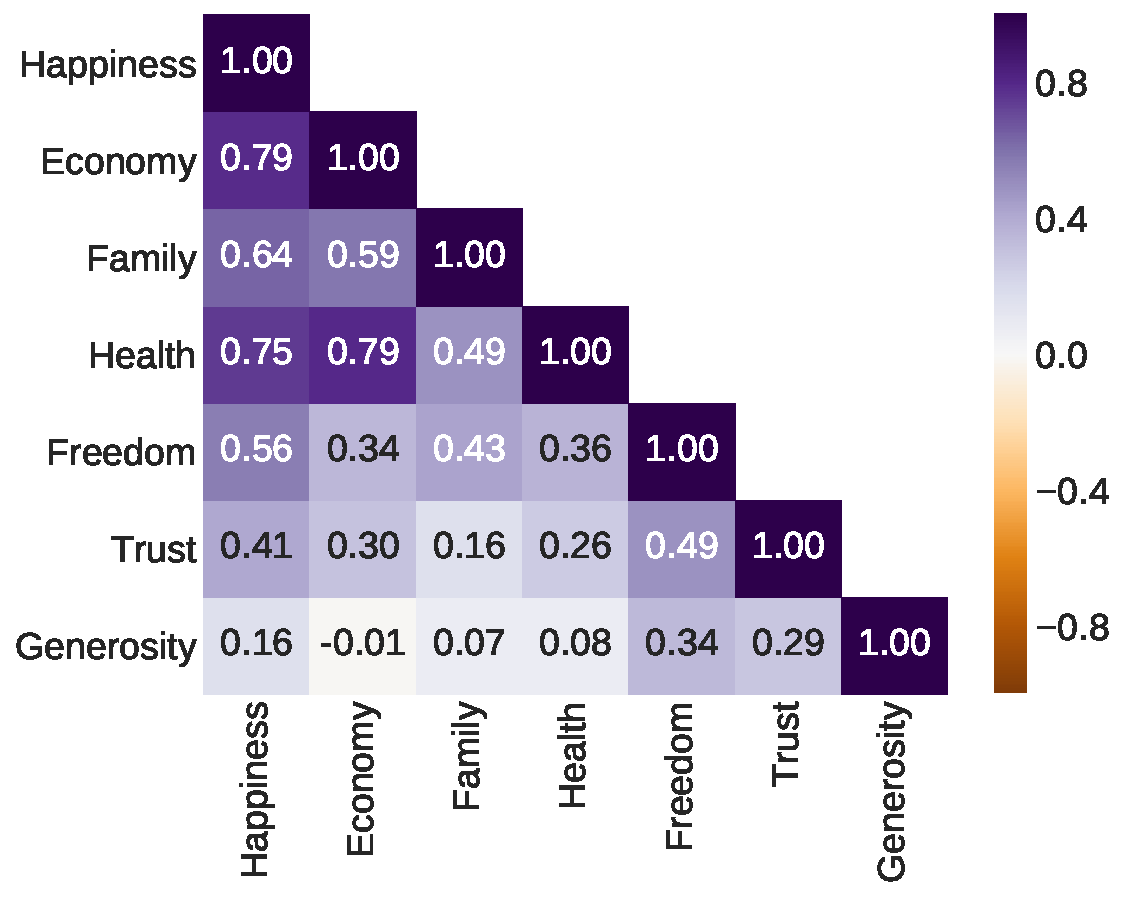
\includegraphics[scale=0.4]{../figs/WH_corr_mat.pdf}
    \caption{Heatmap showing the correlation matrix of the WHR data. The first column shows the correlation with the happiness score, the quantity we wish to predict.}
    \label{fig:WH_corr}
\end{figure}


\begin{figure*}[ht!]
    \centering
    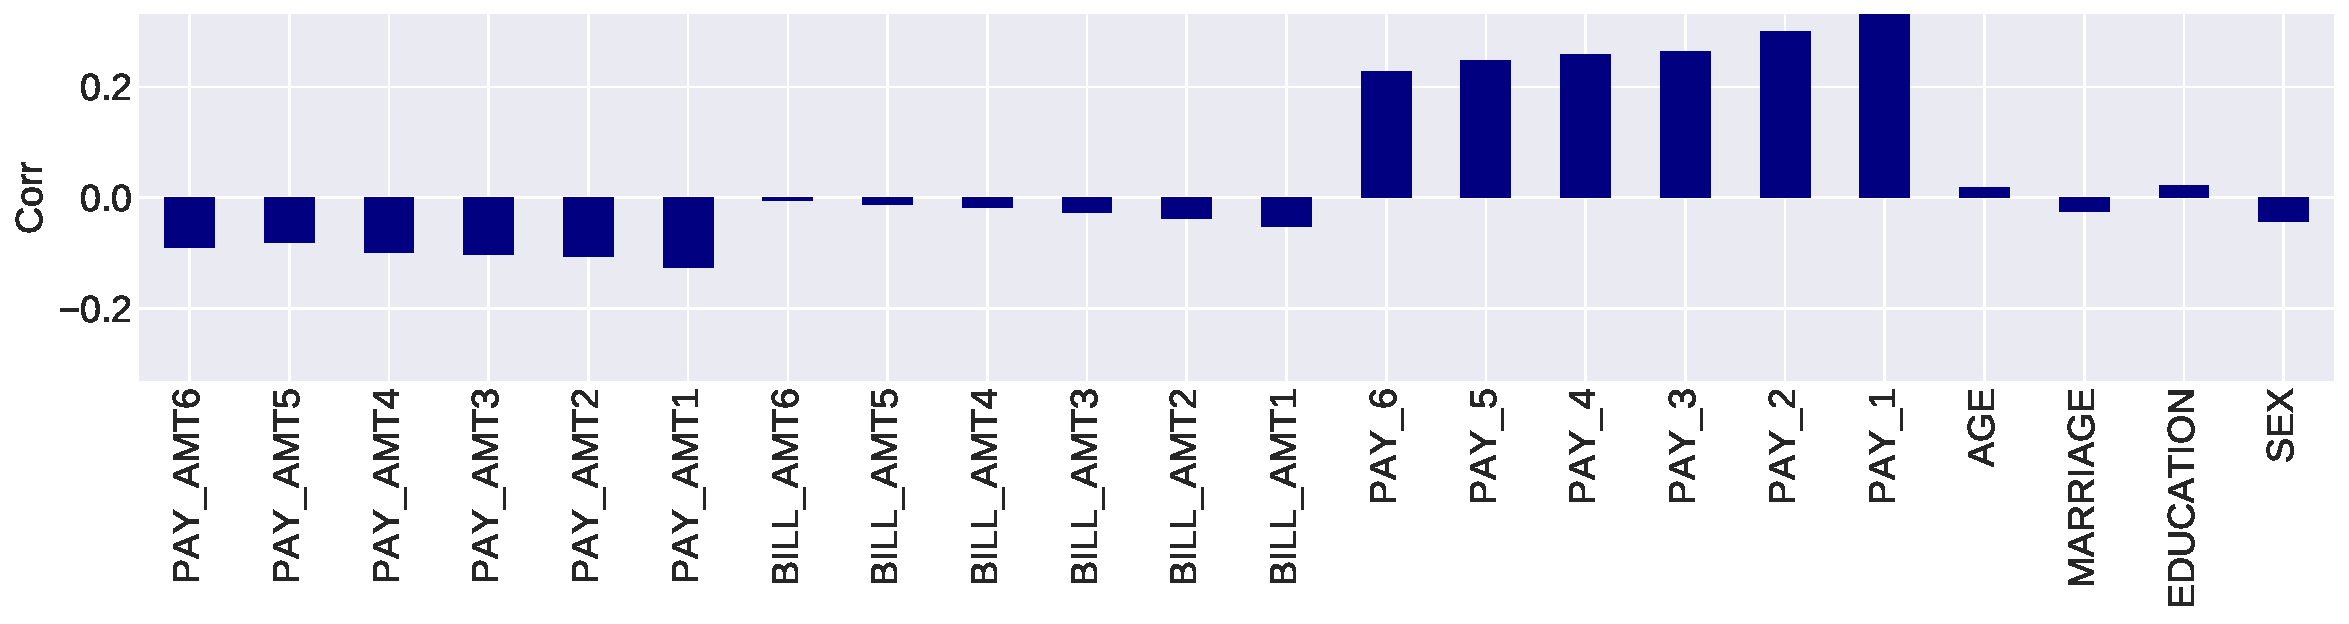
\includegraphics[scale=0.4]{../figs/CC_corr_bars.pdf}
    \caption{Figure showing the correlation between defaulting on credit card depth, and the explanatory variables.}
    \label{fig:CC_corr_bars}
\end{figure*}

\subsubsection{Credit Card data}
Outlier removal, as outlined in \cref{sec:data_cleaning}, was performed on the credit card data. This reduced the total number of data points from 30'000 to 21'308. As this is still a very respectable size for a dataset, and in no way a problematic reduction, no further attempt at making smaller and more surgical reductions was done. The reduction also had the fortunate effect of reducing the fraction of defaulting cases from 0.22 to 0.25, making the data slightly less biased towards not defaulting. It is, however important to keep in mind this bias, as any model simply guessing that nobody will default, will be right 75\% of the time. In the appendix, figures \ref{fig:app1}, \ref{fig:app2}, \ref{fig:app3}, and \ref{fig:app4} can be found, showing the cuts performed, and the reamdining data.

Figure \ref{fig:CC_corr_bars} show the correlation between the default variable (valued 1 for defaulting and 0 for not defaulting) and the 23 explanatory variables. The most correlated quantities are the payment status, which measures the delay on the payment, in months (or -1 for no delay). The payment status is positively correlated with defaulting, saying that a delayed payment gives a more likely default. The payback amount on the bills is negatively correlated with default, meaning that those who pay more back each month are less likely to default. The credit limit is also negatively correlated with default, meaning people who have been given a higher credit limit is less likely to default. The remaining variables are very weakly correlated, and probably within the margin of error. Another natural observation is that, for the columns which spans several months, the later months (like PAY\_1) are more strongly correlated than earlier months. None of these correlations are unexpected or seem unnatural.

The (very large) full correlation matrix, \cref{fig:CC_corr_all}, can be found in the appendix. 






\subsection{Regression}
\subsubsection{Establishing a baseline - OLS and Ridge}
Figure \ref{fig:OLS_Ridge} shows the R2 scores of performing OLS and Ridge regression on the WHR dataset, over a series of polynomial orders and $\lambda$s.

We observe that OLS performs best at very low order, the best score coming out at 0.743, which is achieved with a simple linear fit. Probably due to the very limited size of the dataset, OLS actually manages to overfit already from a second order polynomial. Pretty impressive stuff.

Ridge outperforms OLS, capping out at an R2 score of 0.782, which is achieved over a span of several parameters. The optimal seem to be around $\lambda = 10^{-1.5}$, and polynomial order 4 or 5. The fact that Ridge outperforms OLS (and the fact that higher complexity Ridge outperforms lower complexity Ridge) shows that there actually exists higher order relations between the parameters, but, due to the limited size of the dataset, overfitting can run rampant. One of the main advantages of Ridge regression, its resistance to overfitting, is very evident.

We will keep in mind both the scores of 0.743 and 0.782, serving as fair baselines for a very simple, and slightly more sophisticated regression fit, respectively.


\begin{figure}[H]
    \centering
    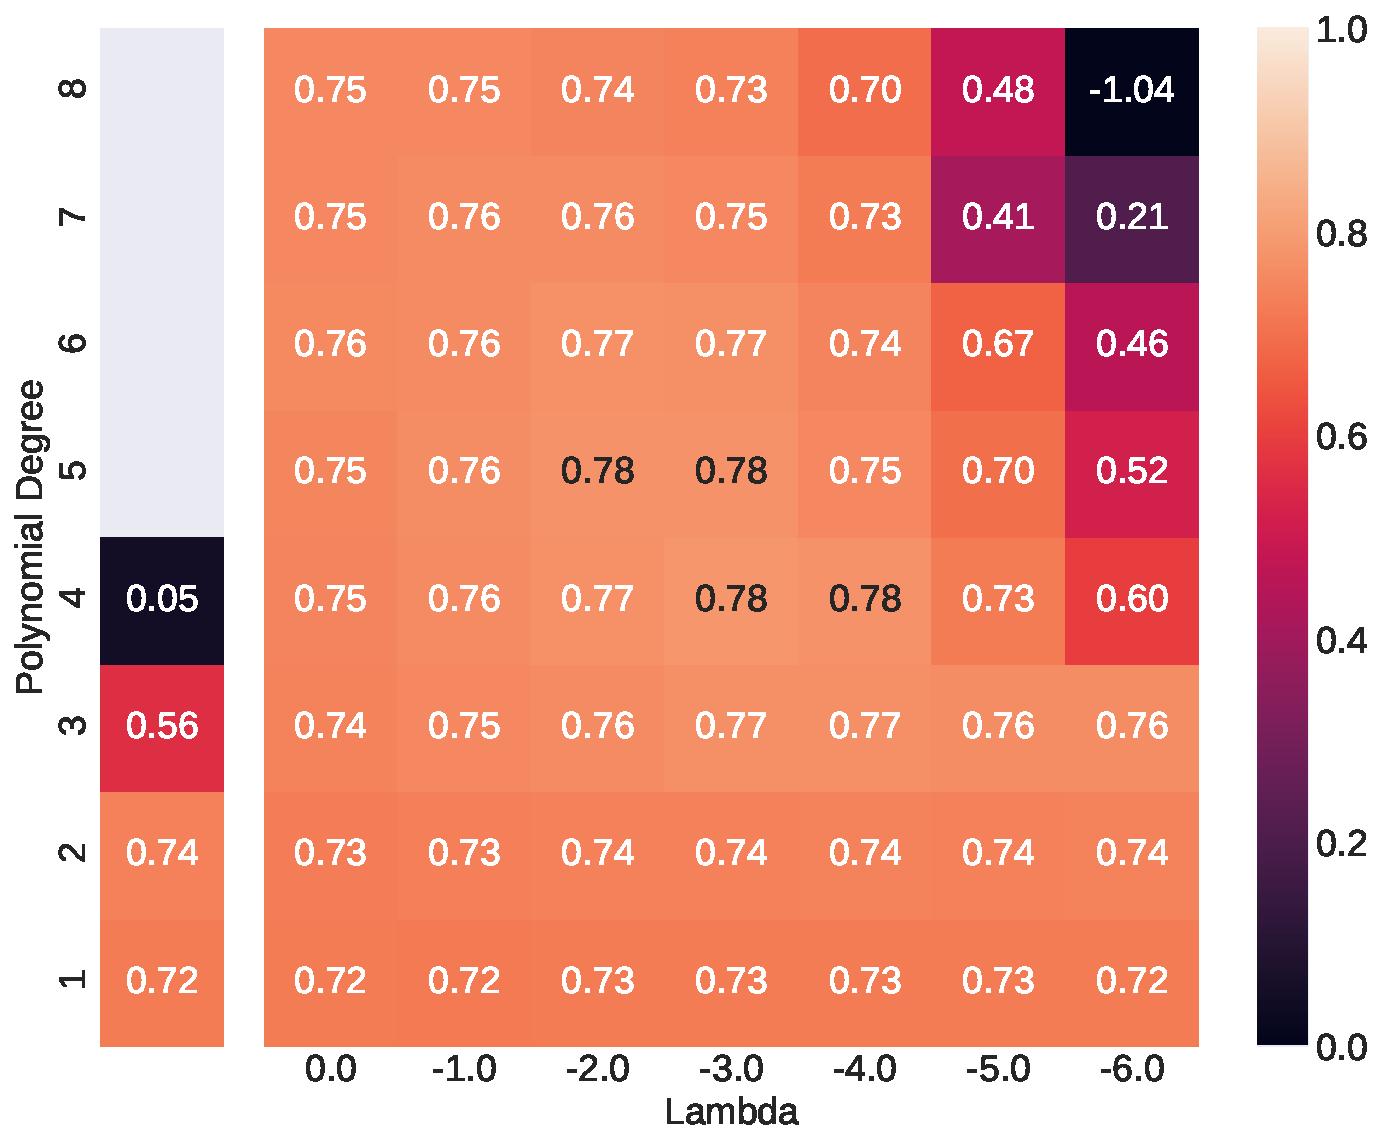
\includegraphics[scale=0.38]{../figs/WH_linreg_r2.pdf}
    \caption{Figure showing R2 score of OLS and Ridge regression as function of polynomial degree and lambda, averaged over 1000 runs. R2 score is calculated on a 10\% randomly selected test data. The column on the right shows the R2 scores of OLS, which doesn't have a lambda value, and only varies with polynomial order. The matrix on the right shows R2 scores of Ridge, which varies both with lambda and polynomial order. Ridge gives the best R2 score, of 0.783, in the region of $\lambda \approx 10^{-2}$, and polynomial order 4-5. OLS performs best for polynomial order 1, with an R2 score of 0.74.}
    \label{fig:OLS_Ridge}
\end{figure}


\subsubsection{Neural Networks}
Figure \ref{fig:WHR_self_TF_comparison} show the R2 score of 10 random runs of our own neural network implementation, and a neural network implementation using Keras, on the WHR regression data. The idea was to confirm that our neural network had expected behavior by comparing it to an identical Keras implementation, before moving forward. The two networks do indeed show very similar behavior, and end up with near identical test data accuracies.\footnote{We have already established the area score as a superior metric to the accuracy score, and we would have prefered to use it. However, we found no simple way of storing it for each epoch in Keras, while this was no problem for the accuracy score. Since we're only trying to confirm the similar behavior of the networks, we found the accuracy score to be adequate.} However, the Keras implementation of the NN seems to learn much quicker, reaching a steady state for the test data very early. It also seem to have much more volatile training accuracy, while the accuracy of both the test data of Keras, and both test and train data on our own network, show a much smoother behavior. We are unsure of what might be causing this, and suspect it might be some techicality buried in the Keras model. Either way, both networks show quantitatively similar behavior, and give very similar results in both training and testing score, and we conclude that our network works as intended.
\begin{figure}[H]
    \centering
    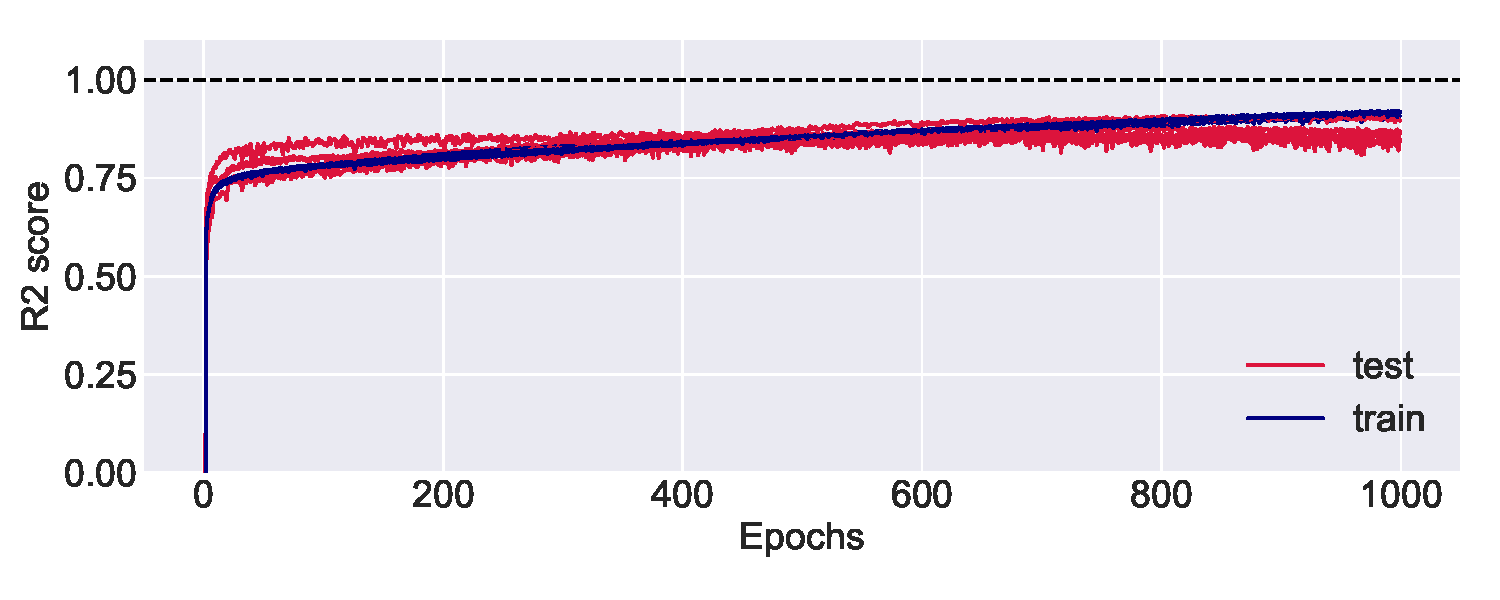
\includegraphics[scale=0.38]{../figs/wh_r2_epochs_self.pdf}
    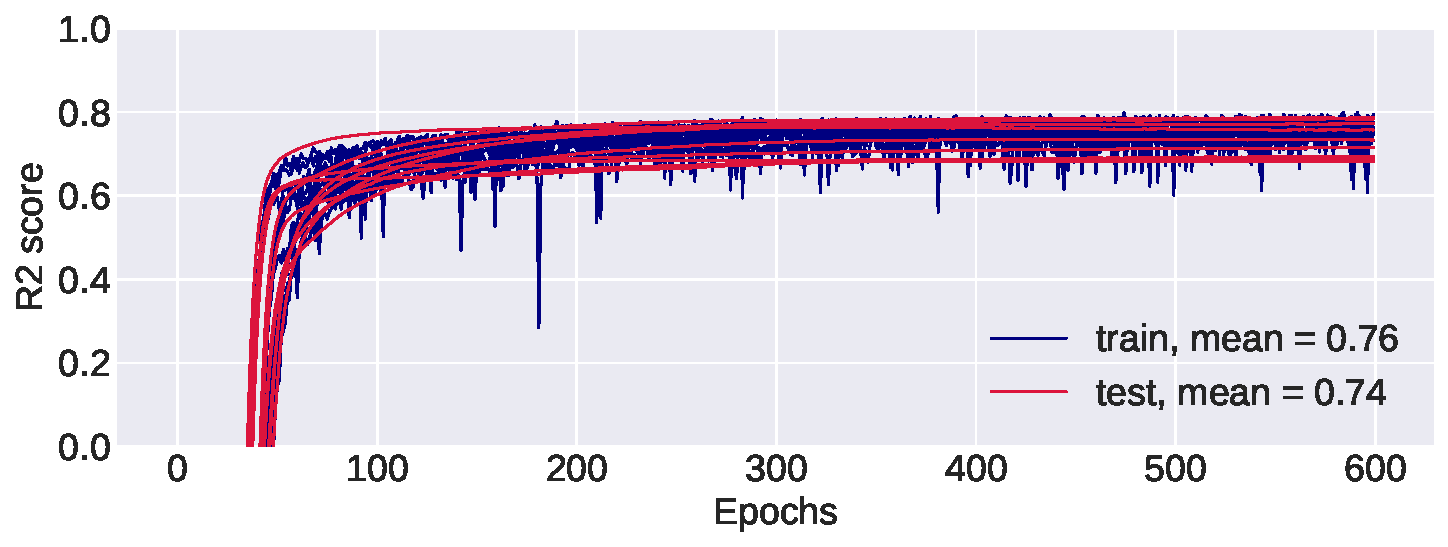
\includegraphics[scale=0.38]{../figs/CC_NN_TF_epochs.pdf}
    \caption{Figure showing the R2 scores of 10 random runs, using a self-built NN (top), and a Keras NN (bottom), trained on the WHR regression data. Both training data, and a randomly selected held-back 30\% testing data, as function of number of epochs, are shown. Both networks employed 2 hidden layers of 16 neurons each, using the ReLu activation, and binary cross entropy loss. Both networks employ the SGD optimizer with a learning rate of $10^{-3}$.}
    \label{fig:WHR_self_TF_comparison}
\end{figure}



\subsubsection{Hyperparameter Optimization}
The hyperparameter optimization on the WHR regression data was performed in Keras, using the parameters outlined in \cref{sec:HP_method}. The 5 best performing networks are shown in \cref{tab:WHR_TF_bestr2}, giving a maximum R2 score of $0.765$. There doesn't appear to be a whole lot of consistence in the types of nerworks that perform the best, as almost every possible value of every hyperparameter shows up in at least one of the five networks.

Figure \ref{fig:WHR_TF_boxplot} shows a somewhat clearer picture, where box plots of the R2 scores, as functions of number of layers and neurons, are shown. While we observe the same thing we observed in the table above - that almost every combination of parameters give \textit{some} results which are promising, some parameters give much more consistenly good results. This specific problem seems to heavily favor narrow networks, with 1 layer performing, on average, much better than more layers do. The network does however seem to favor a higher number of neurons, with 16 and 32 both giving consistently good results.

Figure \ref{fig:WHR_TF_lr_epoch_heatmap} shows the average R2 score of combinations of epochs and learning rate. Since these parameters are expected to be very heavily correlated, they are plotted as a heatmap instead of a boxplot. We observe that the network strongly favors relatively high learning rates, and a high number of epochs. The best results seem to appear with something like 800-1600 epochs, and a learning rate of 0.001.


\begin{table}[H]
    \centering
    \begin{tabular}{R{1.4cm} R{1.6cm} R{1.8cm} R{1.4cm} R{1.2cm}}
        %{\quad \ R2\newline Score} & {\quad \ \ Nr\newline Layers} & {\quad \ \ \ \ Nr\newline Neurons} & {\ \newline LR} & {\ \newline Epochs} \\
        R2 Score & Nr Layers & Nr Neurons & LR & Epochs \\
        \hline
        0.765 & 1 & 16 & 0.00100 & 1600 \\
        \hline
        0.765 & 4 & 16 & 0.01000 & 3200 \\
        \hline
        0.764 & 1 & 8 & 0.00100 & 800 \\
        \hline
        0.762 & 4 & 32 & 0.01000 & 400 \\
        \hline
        0.759 & 1 & 16 & 0.01000 & 3200 \\
        \hline
    \end{tabular}
    \caption{Table showing the 5 best performing neural networks, measured in by R2 score on a held-back 10\% test data, averaged over 40 runs for each combination of hyperparameters.}
    \label{tab:WHR_TF_bestr2}
\end{table}
\newpage 

\begin{figure}[H]
    \centering
    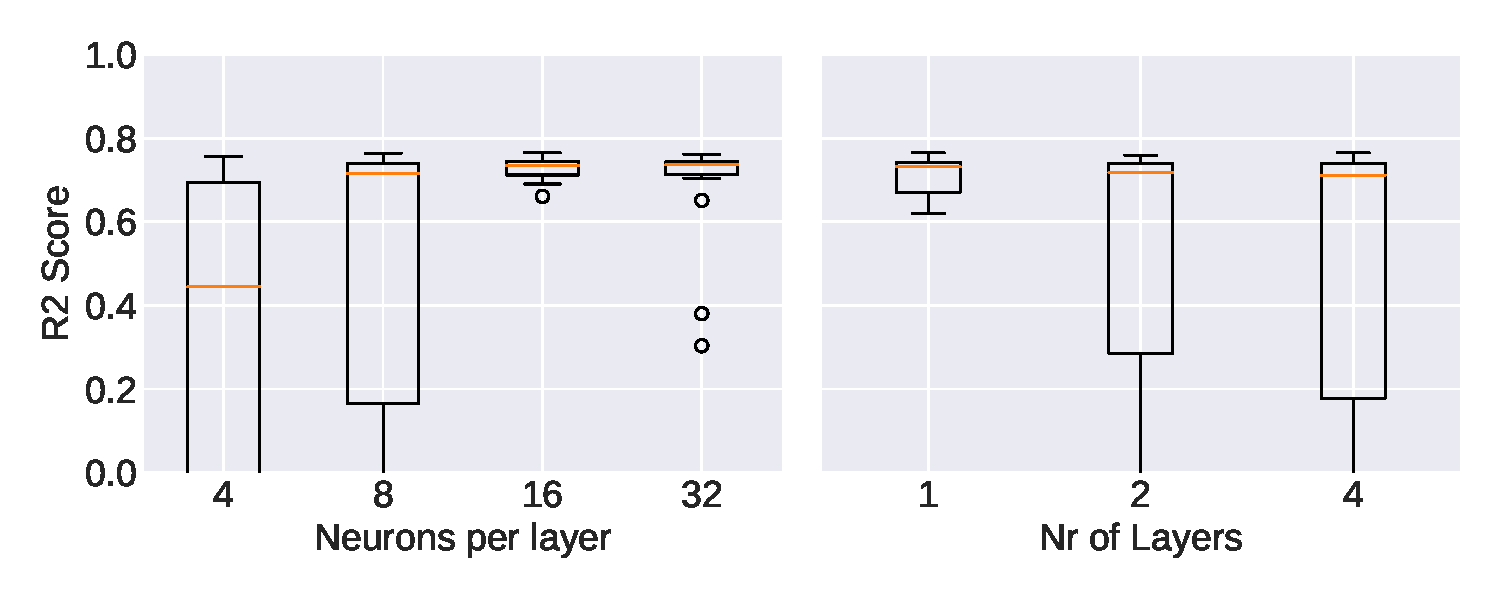
\includegraphics[scale=0.4]{../figs/WHR_TF_boxplot.pdf}
    \caption{Box plots showing the distribution of R2 scores for varying number of neurons per layer, and varying number of layers. Each datapoint represents a unique combinations of hyperparameters, is the average R2 score of a 10\% held-back test data, doing 40 repeated runs using the same hyperparameters.}
    \label{fig:WHR_TF_boxplot}
\end{figure}


\begin{figure}[H]
    \centering
    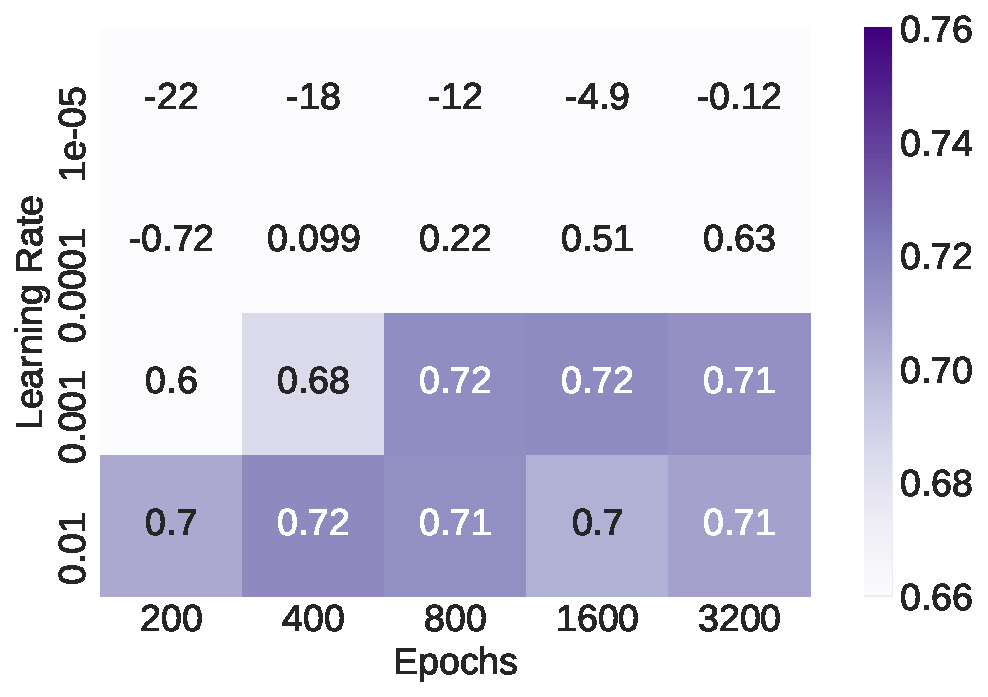
\includegraphics[scale=0.4]{../figs/WHR_TF_lr_epoch_heatmap.pdf}
    \caption{Heatmap showing the R2 score of the neural network fit over a series of epochs and learning rates, averaged over a series of other hyperparameters, as described in \cref{fig:WHR_TF_boxplot}}
    \label{fig:WHR_TF_lr_epoch_heatmap}
\end{figure}


\subsubsection{Comparing the models}
Interestingly, even after a hyperparameter optimization, we are unable to outperform Ridge regression, as seen in \cref{tab:WHR_comparison}. The NN places itself somewhere in the middle of the performance of OLS and Ridge, leaning somewhat more towards the latter. 

\begin{table}[H]
    \centering
    \begin{tabular}{r r r r}
                 & OLS   & Ridge  &  NN \\
                 \hline
    R2 Score     & 0.743 & 0.782  &  0.765
    \end{tabular}
    \caption{Table showing best case R2 score of OLS, Ridge, and NN on 10\% test data.}
    \label{tab:WHR_comparison}
\end{table}

\subsection{Classification}
\subsubsection{Logistic Regression}
Figure \ref{fig:CC_logreg_acc_area} show the area score and accuracy score of the logistic regression classification, as a function of learning rate and number of epochs. We see that the best area and accuracy scores are, respectively, 0.684 and 0.790.

Remembering that a naive model guessing nobody will default gives an accuracy of 0.75, our score of 0.79 might not seem awfully impressive. The accuracy score is, however, not a great metric for performance. A completely naive model would have an area score of 0.5, which makes our score of 0.684 look at least like a fair improvement.

The figures also show that the area score performs very well at low learning rates, and low number of epochs, while the accuracy score performs best at high learning rates, and high number of epochs. They actually seem to be somewhat perfectly inverse, one performing well where the other struggles. This is extremely puzzling, as they should both, to some degree, indicate the performance of the classification. Area score is usually considered a better metric than accuracy, so one should think that the logistic regression performs worse the longer it trains. Often, this would indicate overfitting. However, a logistic regression model has extremely low complexity, and we find it unbelievable that is should be capable of overfitting a dataset of 20'000 points with 24 parameters.

An alternative explanation is that the cost function, which is in the end what we're minimizing, is biased towards higher accuracy, at the expense of area score. We do, however, find this somewhat hard to believe, since our cost function, binary cross entropy, seems better aligned with the area score than it does the accuracy score. In the end, we have no good explanation for this odd result.

\begin{figure}[h]
    \centering
    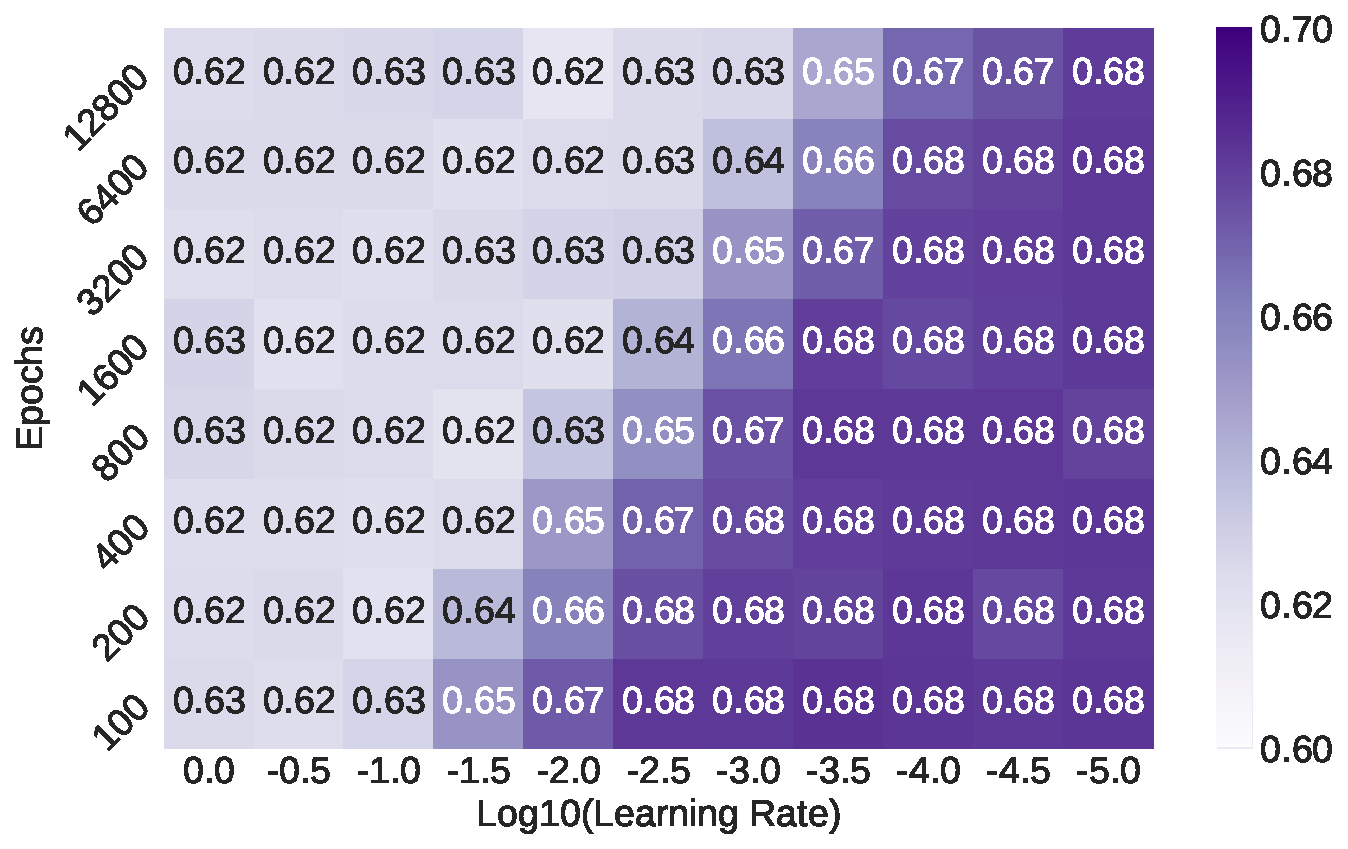
\includegraphics[scale=0.4]{../figs/CC_logreg_area.pdf}
    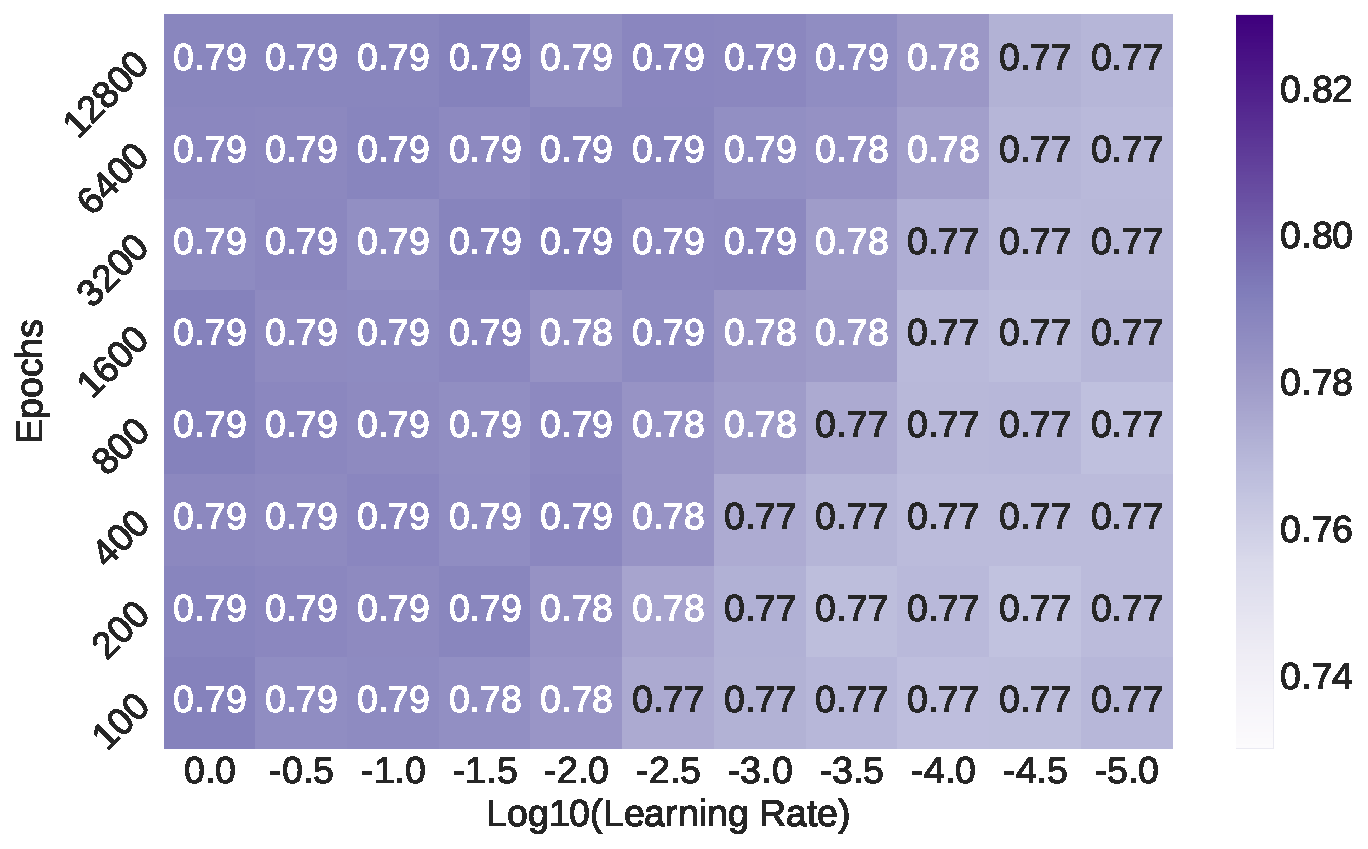
\includegraphics[scale=0.4]{../figs/CC_logreg_acc.pdf}
    \caption{Heatmap showing area score (top) and accuracy score (bottom) of the logistic regression fit over combinations of learning rate and number of epochs used in training. The area score is calculated on a held-back 10\% test data, and is averaged over 40 runs of randomly split train and test datasets.}
    \label{fig:CC_logreg_acc_area}
\end{figure}

 
\subsubsection{Neural Networks}
The results of applying our home-made neural network, as well as a Keras implementation to the credit card classification dataset, is shown in \cref{fig:CC_epochs}. We see that both networks, in all 10 runs shown, converge relatively rapidly to an accuracy somewhere slightly below 0.8. We remember from the logistic regression results that we got an optimal accuracy score of 0.79, which seems in line with what we're seeing here.

The Keras implementation converges quicker than the home-made NN. This is probably due to the usage of a more sophisticated optimizer (Adam vs SGD), because we had problems getting the Keras implementation to play nicely with SGD in the classification case\footnote{It refused to learn properly, and gave terrible results}. It also seem to start out at a higher accuracy, which might be because the first point on the graph is calculated \textit{after} the first epoch, after which the Adam optimizer might already have gained a lot of accuracy. It might also be due to different initialization techniques for the weights and biases.

The plots do, however, look qualitatively similar, and our neural network implementation seems to be working fine.


\begin{figure}[h]
    \centering
    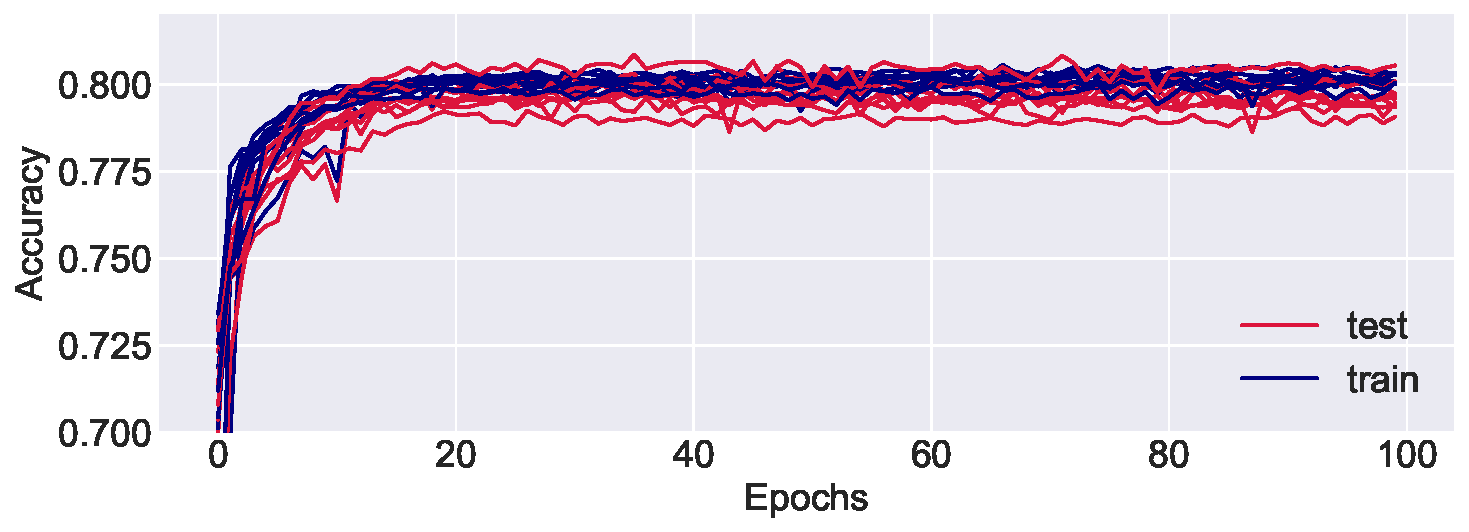
\includegraphics[scale=0.4]{../figs/cc_epochs_self.pdf}
    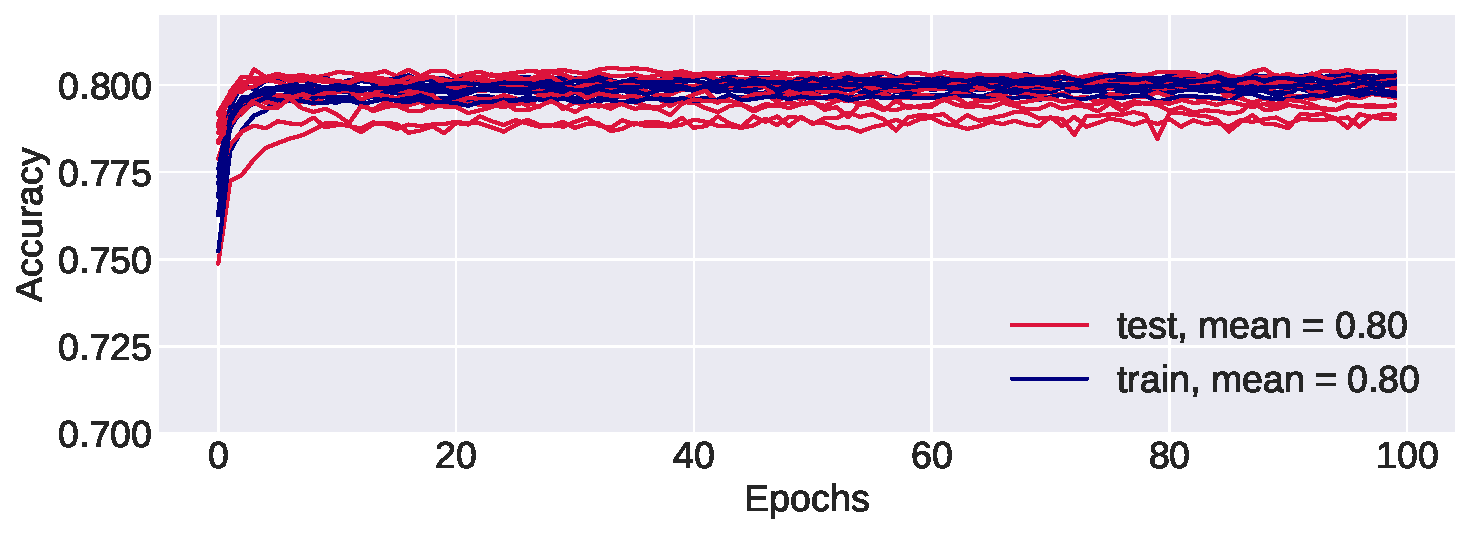
\includegraphics[scale=0.4]{../figs/CC_epochs_TF.pdf}
    \caption{Figure showing the accuracy scores of 10 random runs, using a self-built NN (top), and a Keras NN (bottom), trained on the credit card classification data. Both training data, and a randomly selected held-back 30\% testing data, as function of number of epochs, are shown. Both networks employed 2 hidden layers of 16 neurons each, using the ReLu activation, binary cross entropy loss, and a learning rate of $10^{-3}$. For the self-made NN, the SGD optimizer was used, while the Keras NN employed the more sophisticated Adam optimizer.}
    \label{fig:CC_epochs}
\end{figure}


\subsubsection{Hyperparameter optimization}
The hyperparameter optimization on the CC classification data was performed in Keras, using the parameters outlined in \cref{sec:HP_method}. The 5 best performing networks are shown in \cref{tab:HP_CC}, where we see that the best network performs an area score of 0.670, and an accuracy score of 0.799. We see that among the 5 best networks, every single one has 4 layers, and seem to prefer 16 nodes per layer. 50 epochs also seem to be the preference in these networks, while the learning rate is a bit all over the place.
\begin{table}[H]
    \centering
    \begin{tabular}{R{1cm} R{1cm} R{1cm} R{1.1cm} R{1cm} R{1cm}}
        {\, Area\newline Score} & {\ Acc\newline Score} & {\quad \ Nr\newline Layers} & {\quad \ \ \ \ Nr\newline Neurons} & {\ \newline LR} & {\ \newline Epochs} \\
        \hline
        0.670 & 0.799 & 4 & 16 & 0.0100 & 50 \\
        \hline
        0.667 & 0.797 & 4 & 16 & 0.0010 & 50 \\
        \hline
        0.666 & 0.799 & 4 & 32 & 0.0001 & 50 \\
        \hline
        0.666 & 0.798 & 4 & 16 & 0.0001 & 50 \\
        \hline
        0.664 & 0.797 & 4 & 8 & 0.0010 & 100 \\
        \hline
        
    \end{tabular}
    \caption{Table showing the 5 best performing classification neural networks, measured by their accuracy and area scores, on a held-back 10\% test data, averaged over 40 runs for each combination of hyperparameters.}
    \label{tab:HP_CC}
\end{table}

Figure \ref{fig:HP_neurons_layers_CC} contains a box plot of area scores, over a series of different numbers of layers and neurons per layer. As observed in the table, we see that the best results are obtained with 4 layers, although it should be noted that the 2 layer model contains significantly fewer low outliers. Both 8, 16, and 32 neurons per layer seems to perform fine, but 16 outperforms the other two options by a small margin. It is very interesting to observe that, unlike the regression case, which strongly preferred a shallow network of only 1 hidden layer, the classification case prefers deeper networks, of 4 (or perhaps more) layers.

Figure \ref{fig:HP_epochs_lrs} shows a heatmap of the average area scores for different combinations of epochs and learning rates. Interestingly, there seems to be very small preference in the learning rate or number of epochs for the classification model. This is in big contrast to the regression model, which suffered heavily for small number of epochs, or too low learning rate. It corresponds well to what we saw in \cref{fig:CC_epochs}, namely that the classification neural network converges very quickly.



\begin{figure}[H]
    \centering
    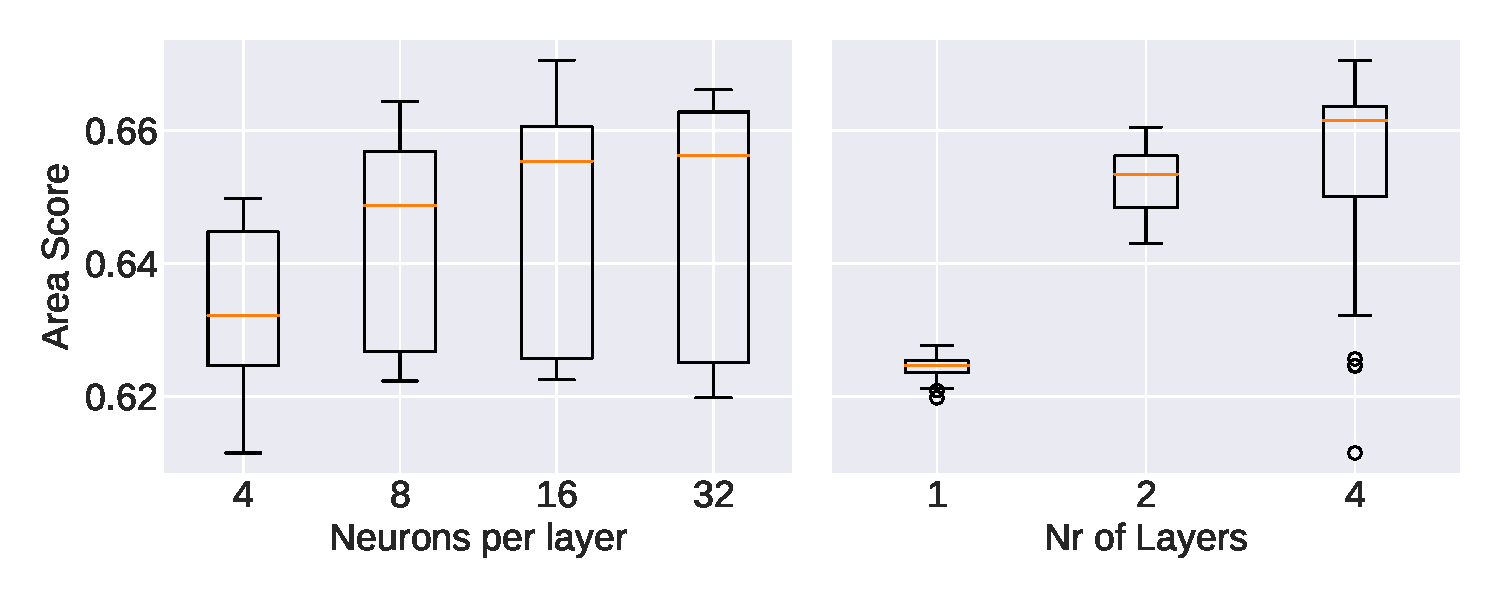
\includegraphics[scale=0.4]{../figs/CC_TF_boxplot.pdf}
    \caption{Box plots showing the distribution of area scores for varying number of neurons per layer, and varying number of layers. Each individual datapoint represents a unique combinations of hyperparameter, and each datapoint is the average area score of a 10\% held-back test data, doing 40 repeated runs using the same hyperparameters.}
    \label{fig:HP_neurons_layers_CC}
\end{figure}

\begin{figure}[H]
    \centering
    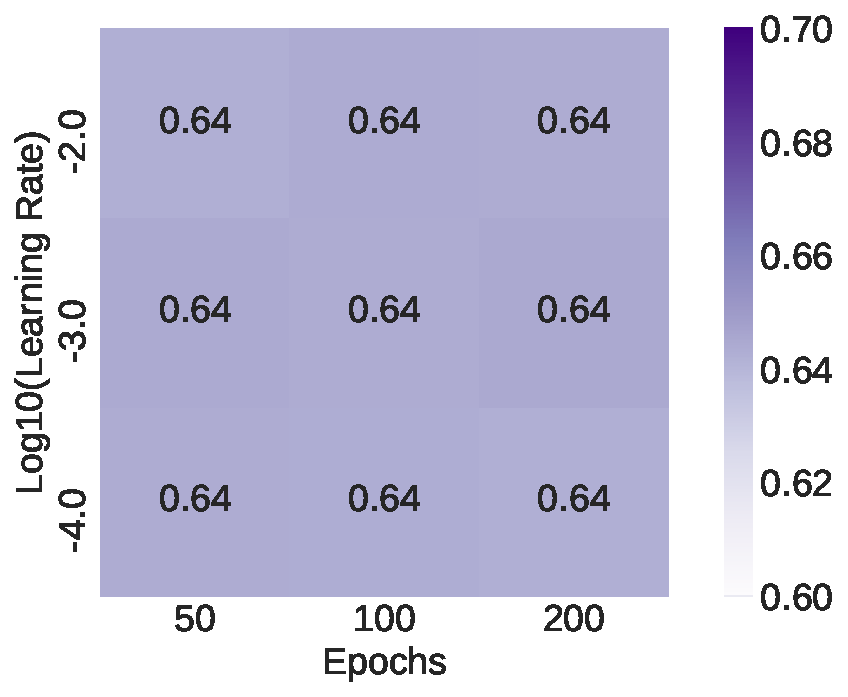
\includegraphics[scale=0.38]{../figs/CC_TF_lr_epoch_heatmap.pdf}
    \caption{Heatmap showing the area scores for combinations of epochs and learning rates, with identical setup as \cref{fig:HP_neurons_layers_CC}}
    \label{fig:HP_epochs_lrs}
\end{figure}
\subsubsection{Comparing the models}
\Cref{tab:CC_comparison} shows the accuracy and area score performance of the logistic regression and neural network models on a the credit card data. The performance of the models is strikingly similar, with the logistic regression performing somewhat better in area score, and the neural net somewhat better in accuracy score. Since we have declared the area score to be a superior metric, we conclude that the logistic regression outperforms the neural network, although with a very small margin.
\begin{table}[H]
    \centering
    \begin{tabular}{r r r}
                 & Log.Reg. &  NN \\
                 \hline
    Acc Score     & 0.790  &  0.799 \\
                 \hline
    Area Score    & 0.684  &  0.670
    \end{tabular}
    \caption{Table showing best case accuracy and area score of logistic regression and NN on 10\% test data.}
    \label{tab:CC_comparison}
\end{table}

\subsection{Timings}
Figure \ref{fig:timings} show the time-usage of the self implemented and Keras implemented networks, over a number of different neurons in each layer. For layer sizes smaller than $\sim100$, our network outperforms Keras by a rather substantial factor. Keras seem to have some minimum runtime, no matter how small the network is, perhaps caused by compilation, or constant overhead on the propagations. For larger sets of neurons, Keras strongly outperforms our network, and probably employs more effective linear algebra operations for large matrices than we are capable of. The networks have equal performance around $\sim100$ neurons per layer.
\begin{figure}[H]
    \centering
    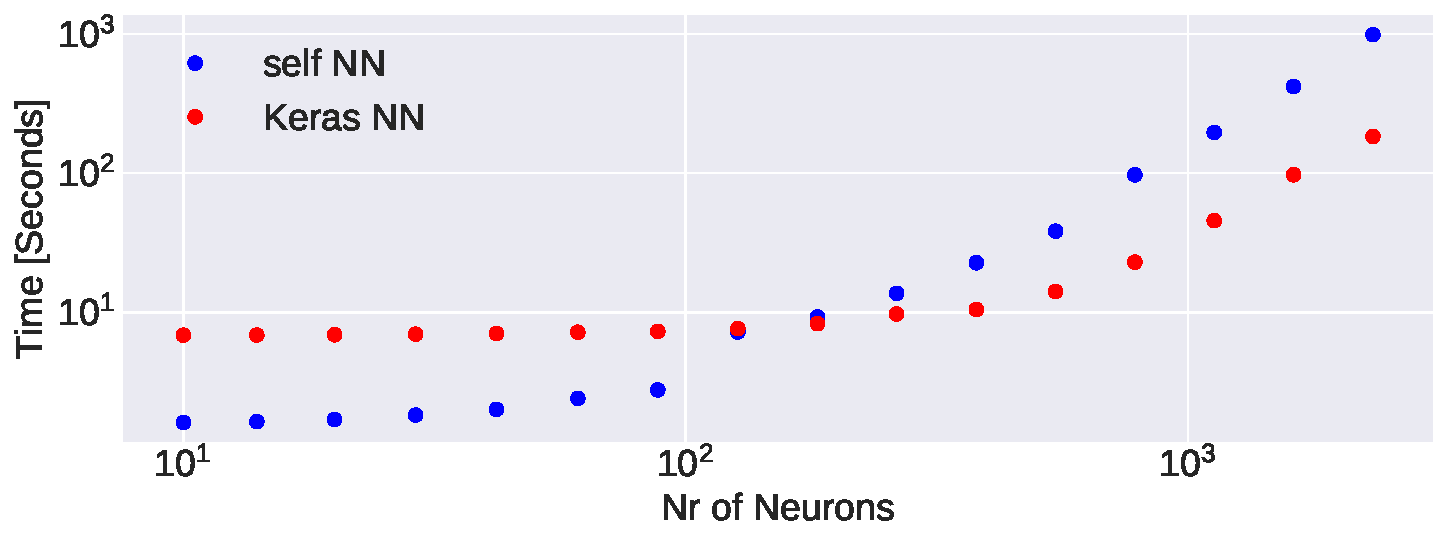
\includegraphics[scale=0.38]{../figs/timings.pdf}
    \caption{Figure showing time usage of training both the self written and Keras implemented regression NNs, using two hidden layers of variable sizes. The WHR dataset is used, with SGD, 1000 epochs and a batch size of 32, and averaged over 20 runs.}
    \label{fig:timings}
\end{figure}




%  ██████╗ ██████╗ ███╗   ██╗ ██████╗██╗     ██╗   ██╗███████╗██╗ ██████╗ ███╗   ██╗
% ██╔════╝██╔═══██╗████╗  ██║██╔════╝██║     ██║   ██║██╔════╝██║██╔═══██╗████╗  ██║
% ██║     ██║   ██║██╔██╗ ██║██║     ██║     ██║   ██║███████╗██║██║   ██║██╔██╗ ██║
% ██║     ██║   ██║██║╚██╗██║██║     ██║     ██║   ██║╚════██║██║██║   ██║██║╚██╗██║
% ╚██████╗╚██████╔╝██║ ╚████║╚██████╗███████╗╚██████╔╝███████║██║╚██████╔╝██║ ╚████║
%  ╚═════╝ ╚═════╝ ╚═╝  ╚═══╝ ╚═════╝╚══════╝ ╚═════╝ ╚══════╝╚═╝ ╚═════╝ ╚═╝  ╚═══╝
\section{Conclusion}
In this project we have explored classification and regression problems, mainly focusing on the performance of neural networks, and logistic regression, to do such tasks. The inner workings of a neural net, and a logistic regression model, was of especial focus, and these models were both explored in theoretical detail, and built from the ground up in Python. For comparison, we employed OLS and Ridge regression from the Scikitlearn package, and a Keras implementation of a neural network. For regression, we studied and employed a dataset on international happiness rankings from the World Happiness Report, 2015-2017. For classification, a dataset on credit card defaults from a Taiwanese bank, 2005, was cleaned, studied, and used.

Both regression and classification showed very similar behavior in the final test data results between our self implemented neural network, and the Keras implementation. The runtime performance of the two implementations showed that our own implementation outperformed Keras in speed for narrow networks (< 100 neurons per layer), while Keras won for broader networks.

In regression, the neural network reached a final R2 score of 0.765, placing it in between the score obtained by OLS, of 0.743, and that of Ridge, of 0.782. The scores were all obtained through hyperparameter optimization of relevant variables, for all three models. The regression problem showed a clear preference for shallow, but broad neural networks, with only one hidden layer, but a large number of nodes.

In classification, the neural network again found itself slightly outperformed by more traditional models. The neural network achieved a area score of 0.670, while logistic regression ended up at 0.684. Again, the hyperparameters of both models were optimized. The classification problem favored deeper neural networks, performing its best at our maximum chosen depth of 4, while favoring a relatively narrow number of 16 neurons per layer.

\subsection{Future Prospects}
In this project we have been given the opportunity to delve deep into the workings of neural networks, both the professional Keras implementation and building our own from the ground up. Unfortunately the development of our own network was slow in the beginning, as we didn't find a good way to benchmark our code before the full network was in place, at which point it obviously was full of bugs. Because of time constraints and us being unsure of when we would get our own network to run, we did the hyperparameter optimization on the network built with Keras. To reduce the amount of results presented in this report we decided to not redo all of this work with our own network, and just compare the networks with the results obtained from the optimization of Keras. We didn't honestly expect our own network to perform inline with the professional tools, and in hindsight it would be really interesting to perform a proper hyperparameter optimization for our own network. Some of the same heatmaps presented here where also produced for our own network, but in a fast and ad-hoc way for fast comparison and benchmarking. In the end these are not included, as we would need a lot more computation time to produce consistent results by averaging over many runs.

As we saw from the timing of our networks in \cref{fig:timings}, it was a pleasant surprise to note that our network actually outperformed Keras on smaller networks, with similar accuracy. We have a lot of future improvements in mind which would be fun and interesting to implement. First of, it would be interesting to optimize the code even further from a run time perspective, starting by optimizing the backward propagation algorithm for speed. Also, as the code is written in a highly modular and object oriented way, as discussed in \cref{subsubsec:Method/Building_NN}, further extension to include more available activation functions and cost functions in the problem classes would be easy to implement. It would also be fun to see the effects of having different activation functions in each hidden layer, especially for networks with high number of layers.

We would also very much have liked to explore a larger set of hyperparameters in our optimizations, particularly for the classification problem. The classification data seemed to prefer deeper networks, but we limited ourselves to four layers in our hyperparameter optimization. A drawback of introducing more layers is that it increases the complexity, and thereby the chance of overfitting. As we saw in \cref{fig:HP_neurons_layers_CC}, while 4 layers gave the overall best results, it also had a significantly larger spread in values than the shallower. A common technique to counter overfitting in neural networks is \textit{regularization}, which involves penalizing large activation on a single node with a new hyperparameter, in a similar concept as Ridge regression does with its introduction of the $\lambda$ hyperparameter. It would have been very interesting to see if we could improve the performance of our classification network by further increasing the number of layers, and in addition, add regularization to the list of optimized hyperparameters, to counter the impact of overfitting, which might become a large problem for even deeper networks.

%  █████╗ ██████╗ ██████╗ ███████╗███╗   ██╗██████╗ ██╗██╗  ██╗
% ██╔══██╗██╔══██╗██╔══██╗██╔════╝████╗  ██║██╔══██╗██║╚██╗██╔╝
% ███████║██████╔╝██████╔╝█████╗  ██╔██╗ ██║██║  ██║██║ ╚███╔╝ 
% ██╔══██║██╔═══╝ ██╔═══╝ ██╔══╝  ██║╚██╗██║██║  ██║██║ ██╔██╗ 
% ██║  ██║██║     ██║     ███████╗██║ ╚████║██████╔╝██║██╔╝ ██╗
% ╚═╝  ╚═╝╚═╝     ╚═╝     ╚══════╝╚═╝  ╚═══╝╚═════╝ ╚═╝╚═╝  ╚═╝
\onecolumn
\bibliography{ref}
\newpage
\begin{appendices}
\section{Figures that didn't make it}

\begin{figure}[h]
    \centering
    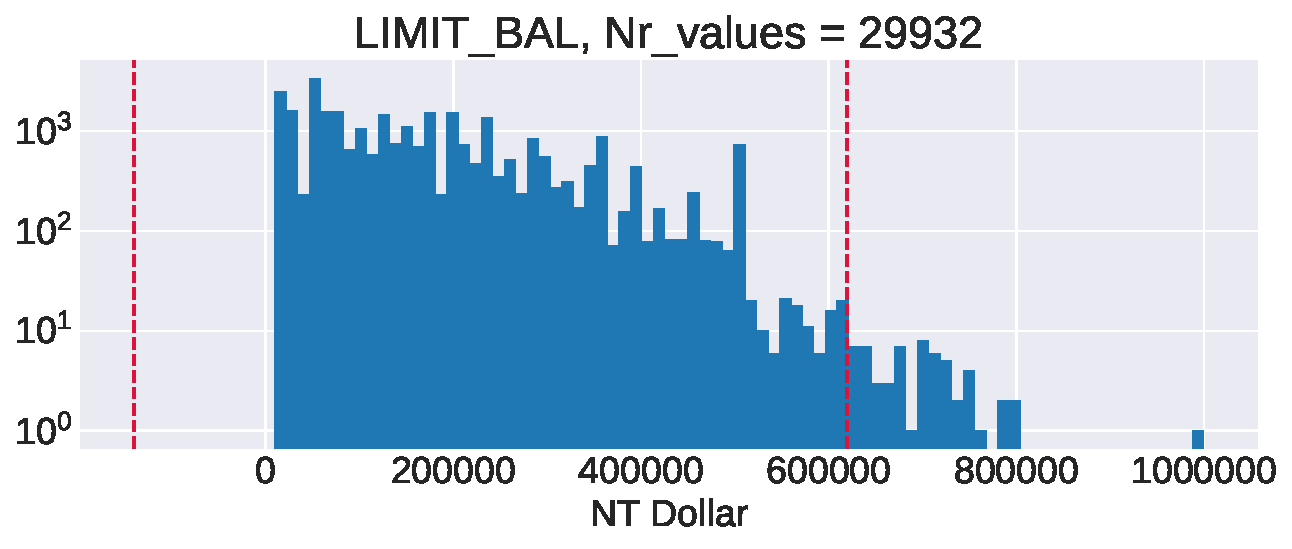
\includegraphics[scale=0.4]{../figs/CC_IQR_cuts_LIMIT_BAL.pdf}
    \caption{Histogram showing the distribution of credit limits, as well as the outlier cuts, as red lines.}
    \label{fig:app1}
\end{figure}

\begin{figure}[h]
    \centering
    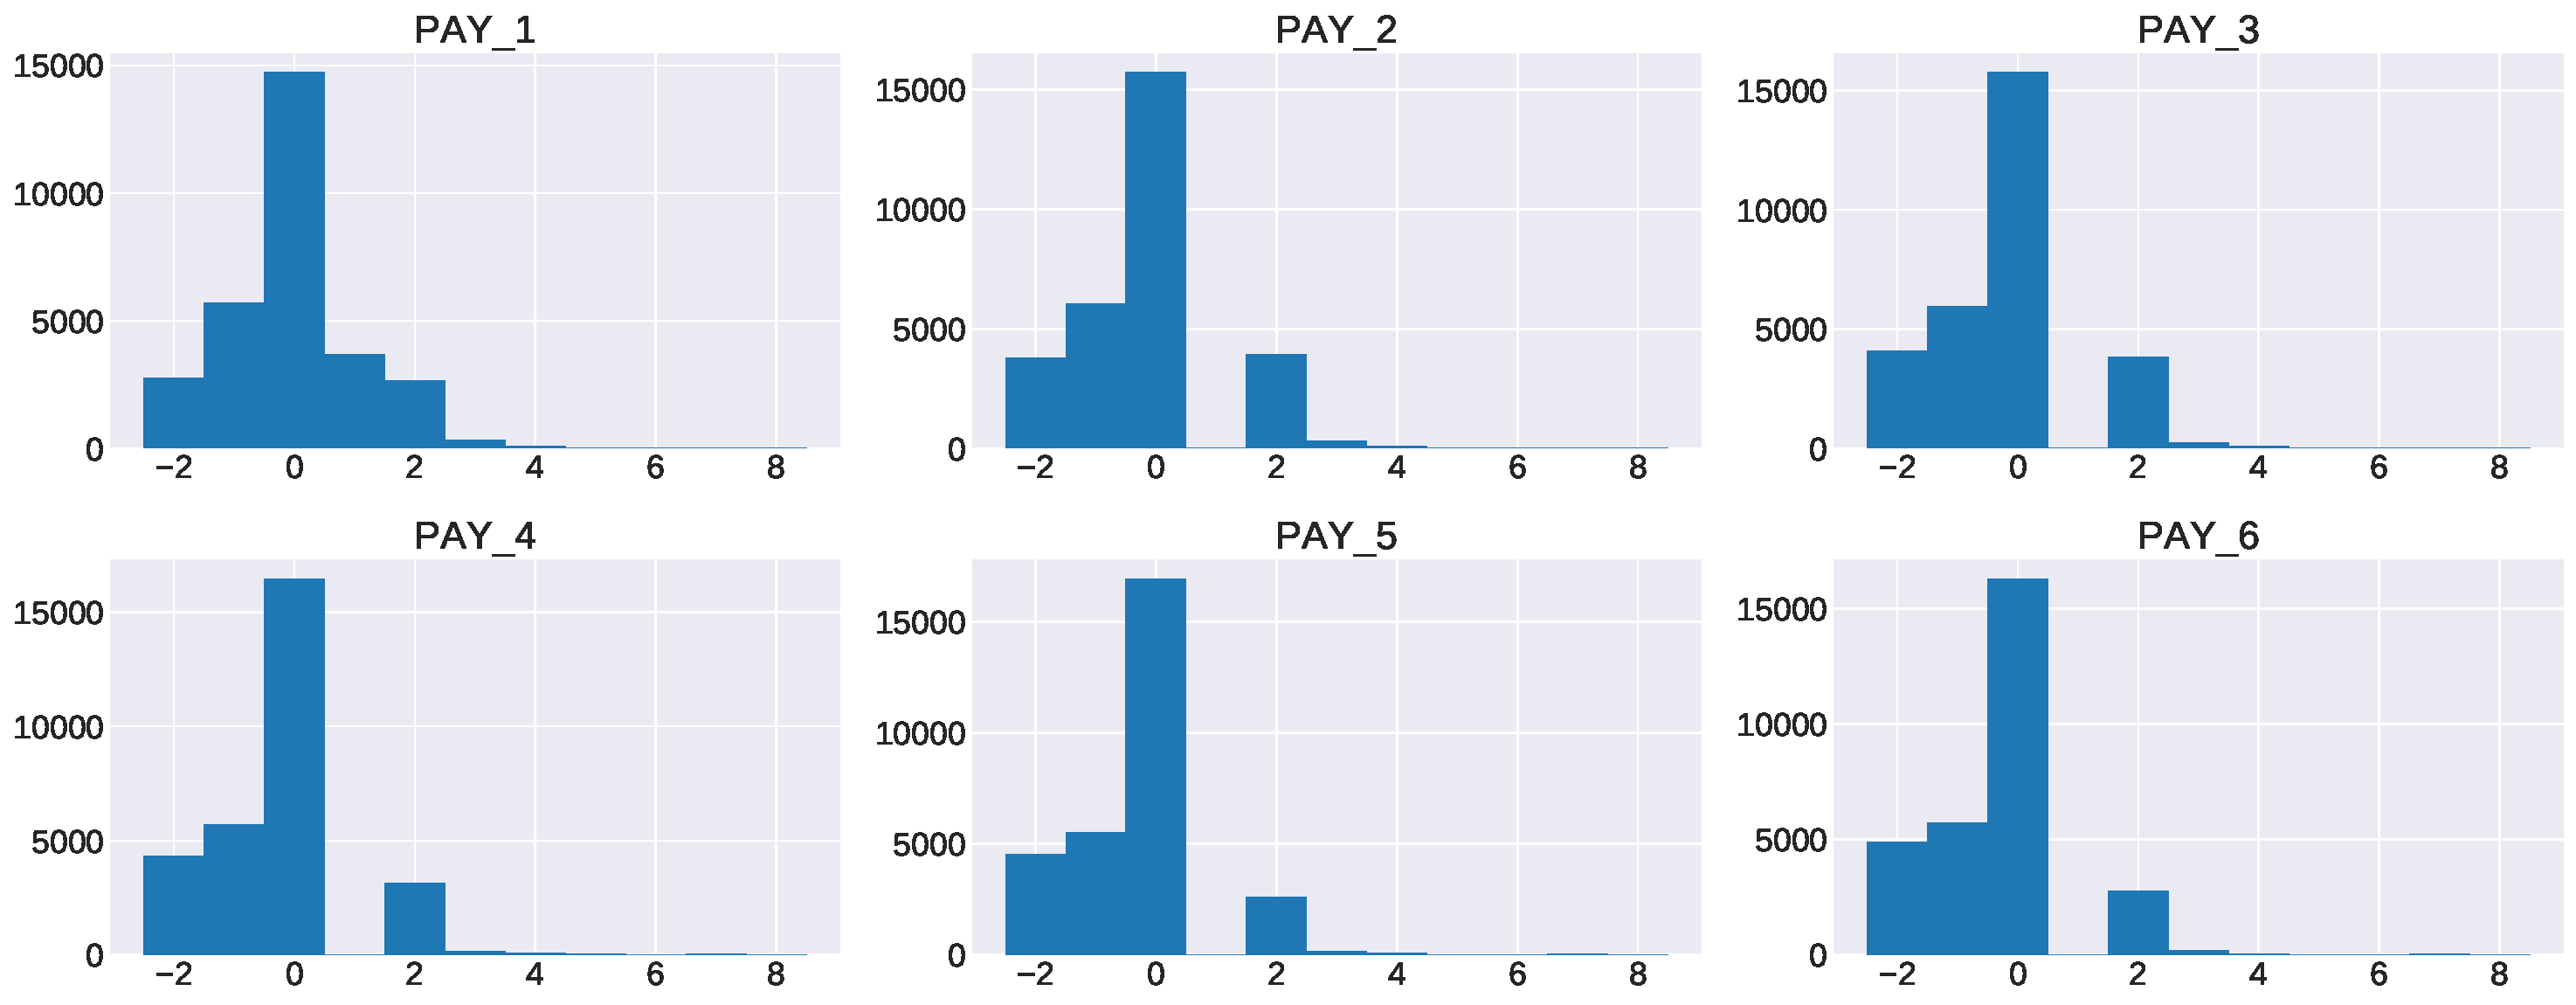
\includegraphics[scale=0.4]{../figs/CC_PAY_hist.pdf}
    \caption{Histogram showing the distribution of payment statuses. Oddly, the value of 1 is missing from every column but PAY\_1. It is unknown why. }
    \label{fig:app2}
\end{figure}

\begin{figure}[h]
    \centering
    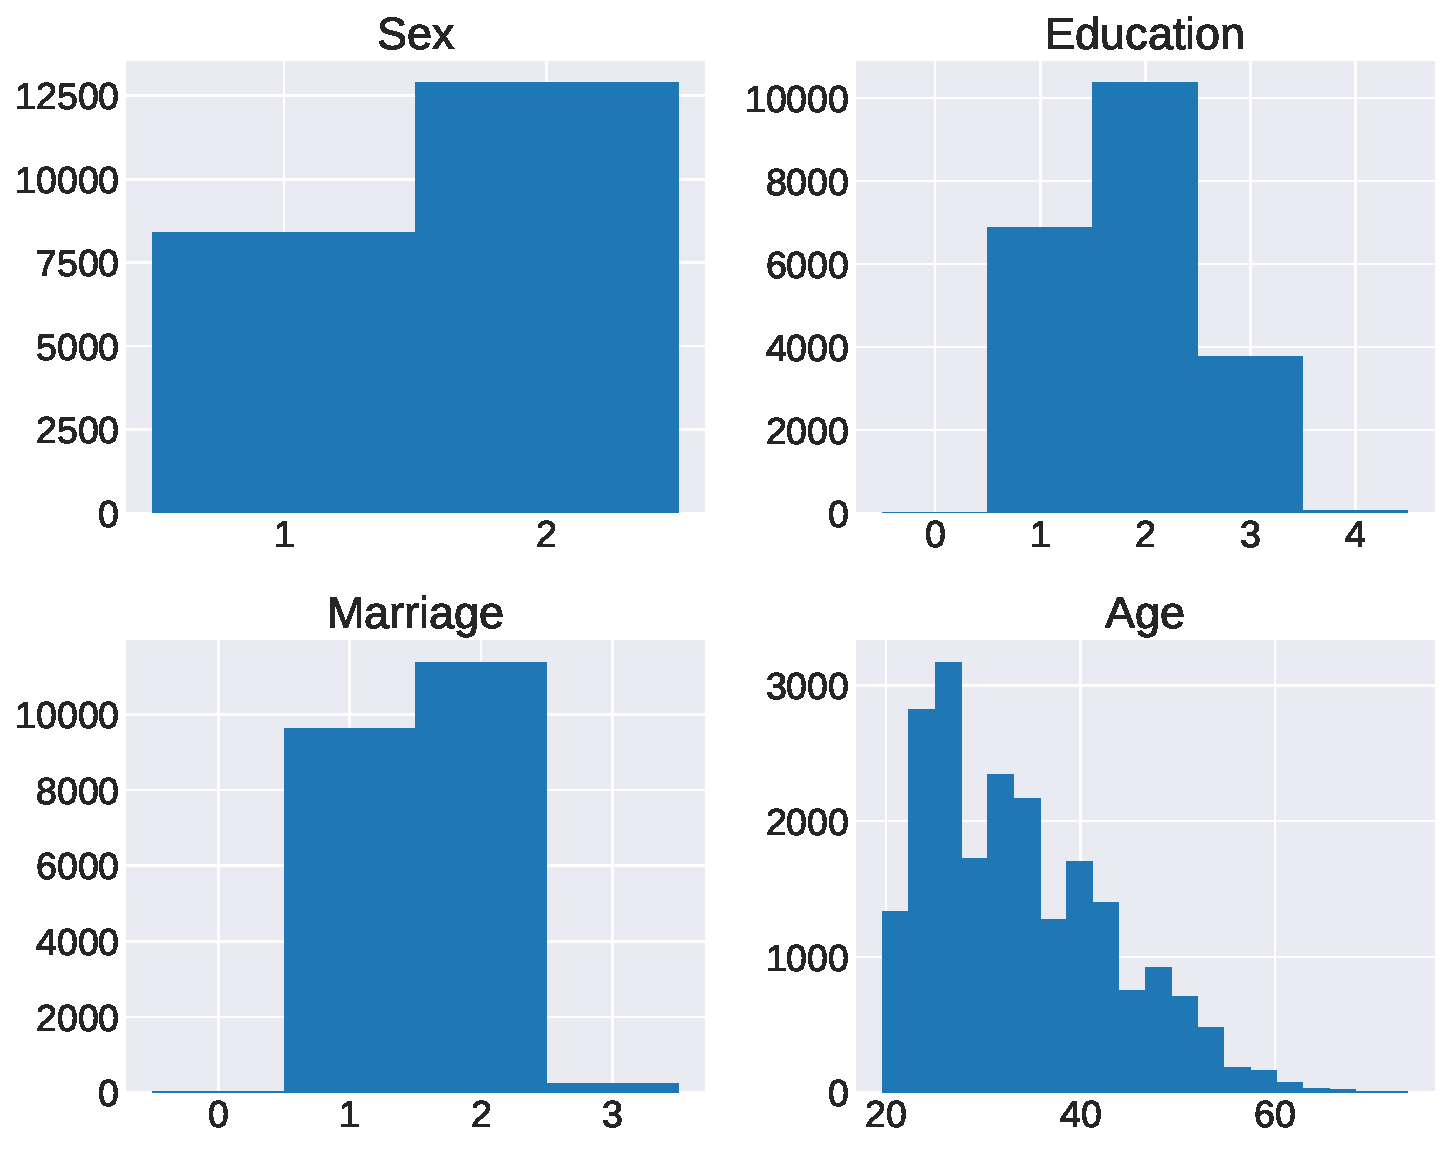
\includegraphics[scale=0.4]{../figs/CC_params_hist.pdf}
    \caption{Histogram showing the distribution of credit limits, as well as the outlier cuts, as red lines.}
    \label{fig:app3}
\end{figure}

\begin{figure}[h]
    \centering
    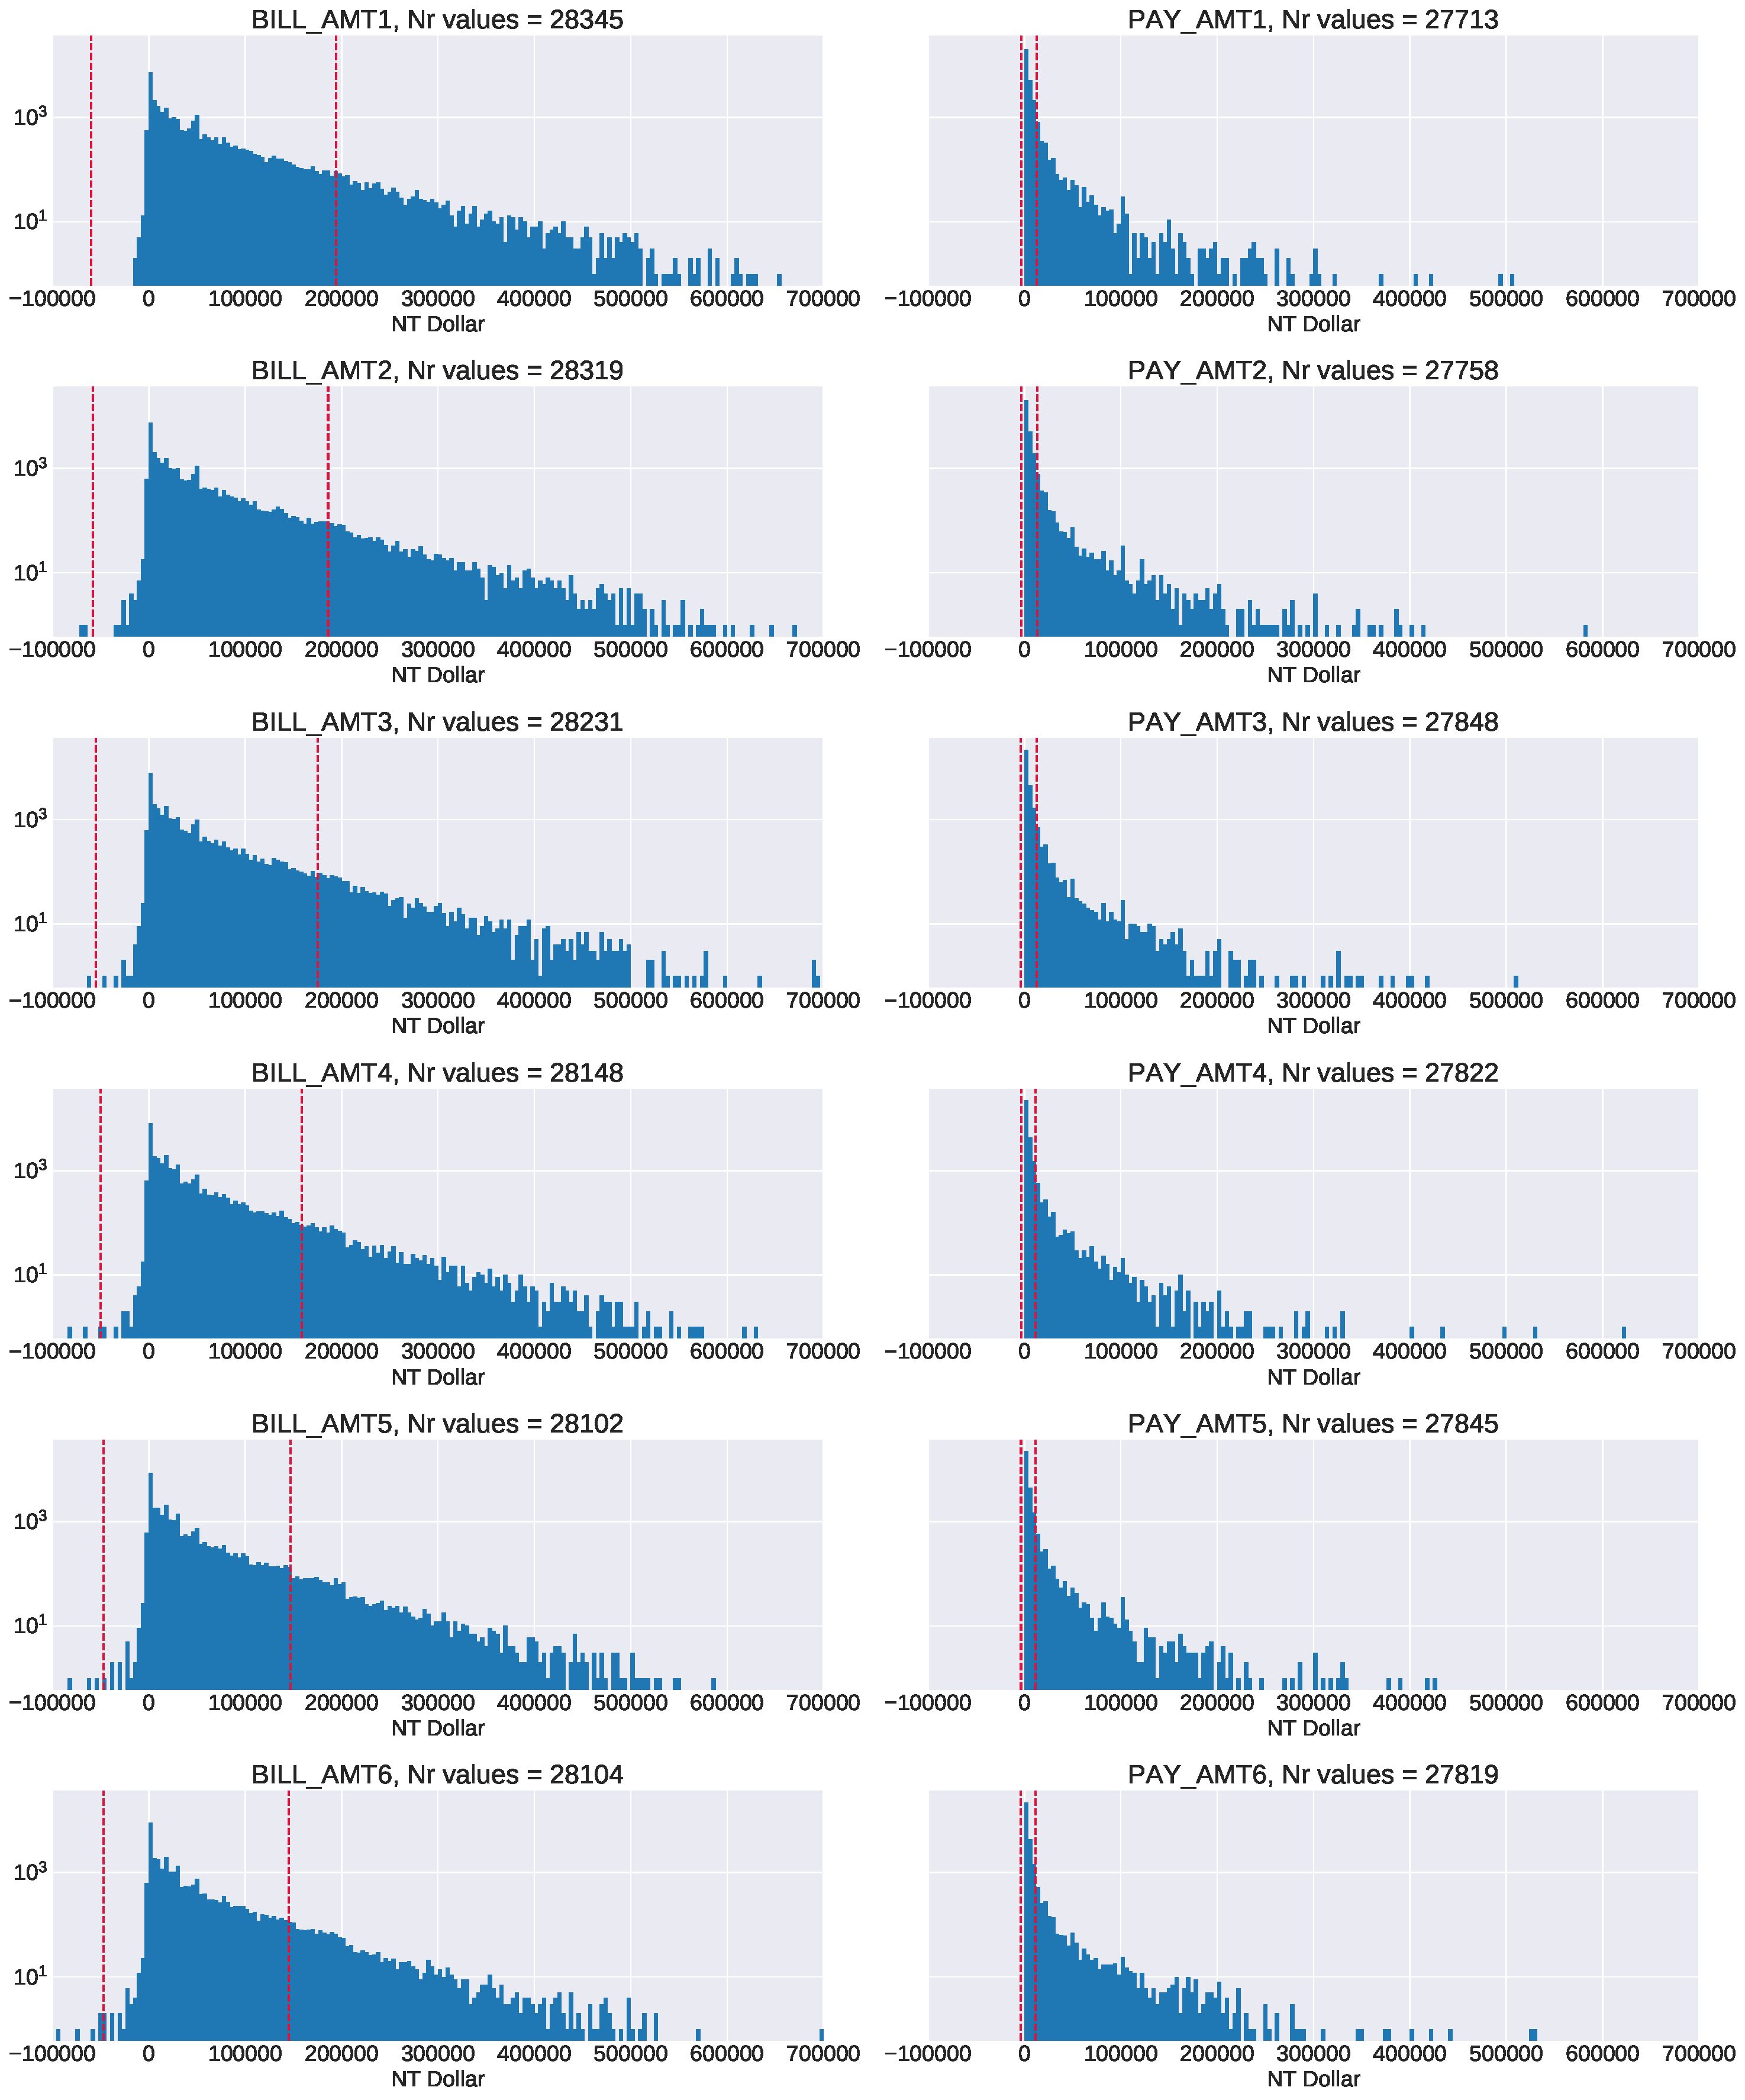
\includegraphics[scale=0.38]{../figs/CC_IQR_cuts_BILL_PAY.pdf}
    \caption{Histograms showing the distributions of values for bill amount (left) and payment amount (right) in the credit card data, as well as the outlier cuts, as red lines. The number of remaining values (down from 30'000) is shown in the title. Keep in mind that the y-axis is logarithmic, so the cuts aren't nearly as invasive as they might seem at first.}
    \label{fig:app4}
\end{figure}


\begin{figure}[h]
    \centering
    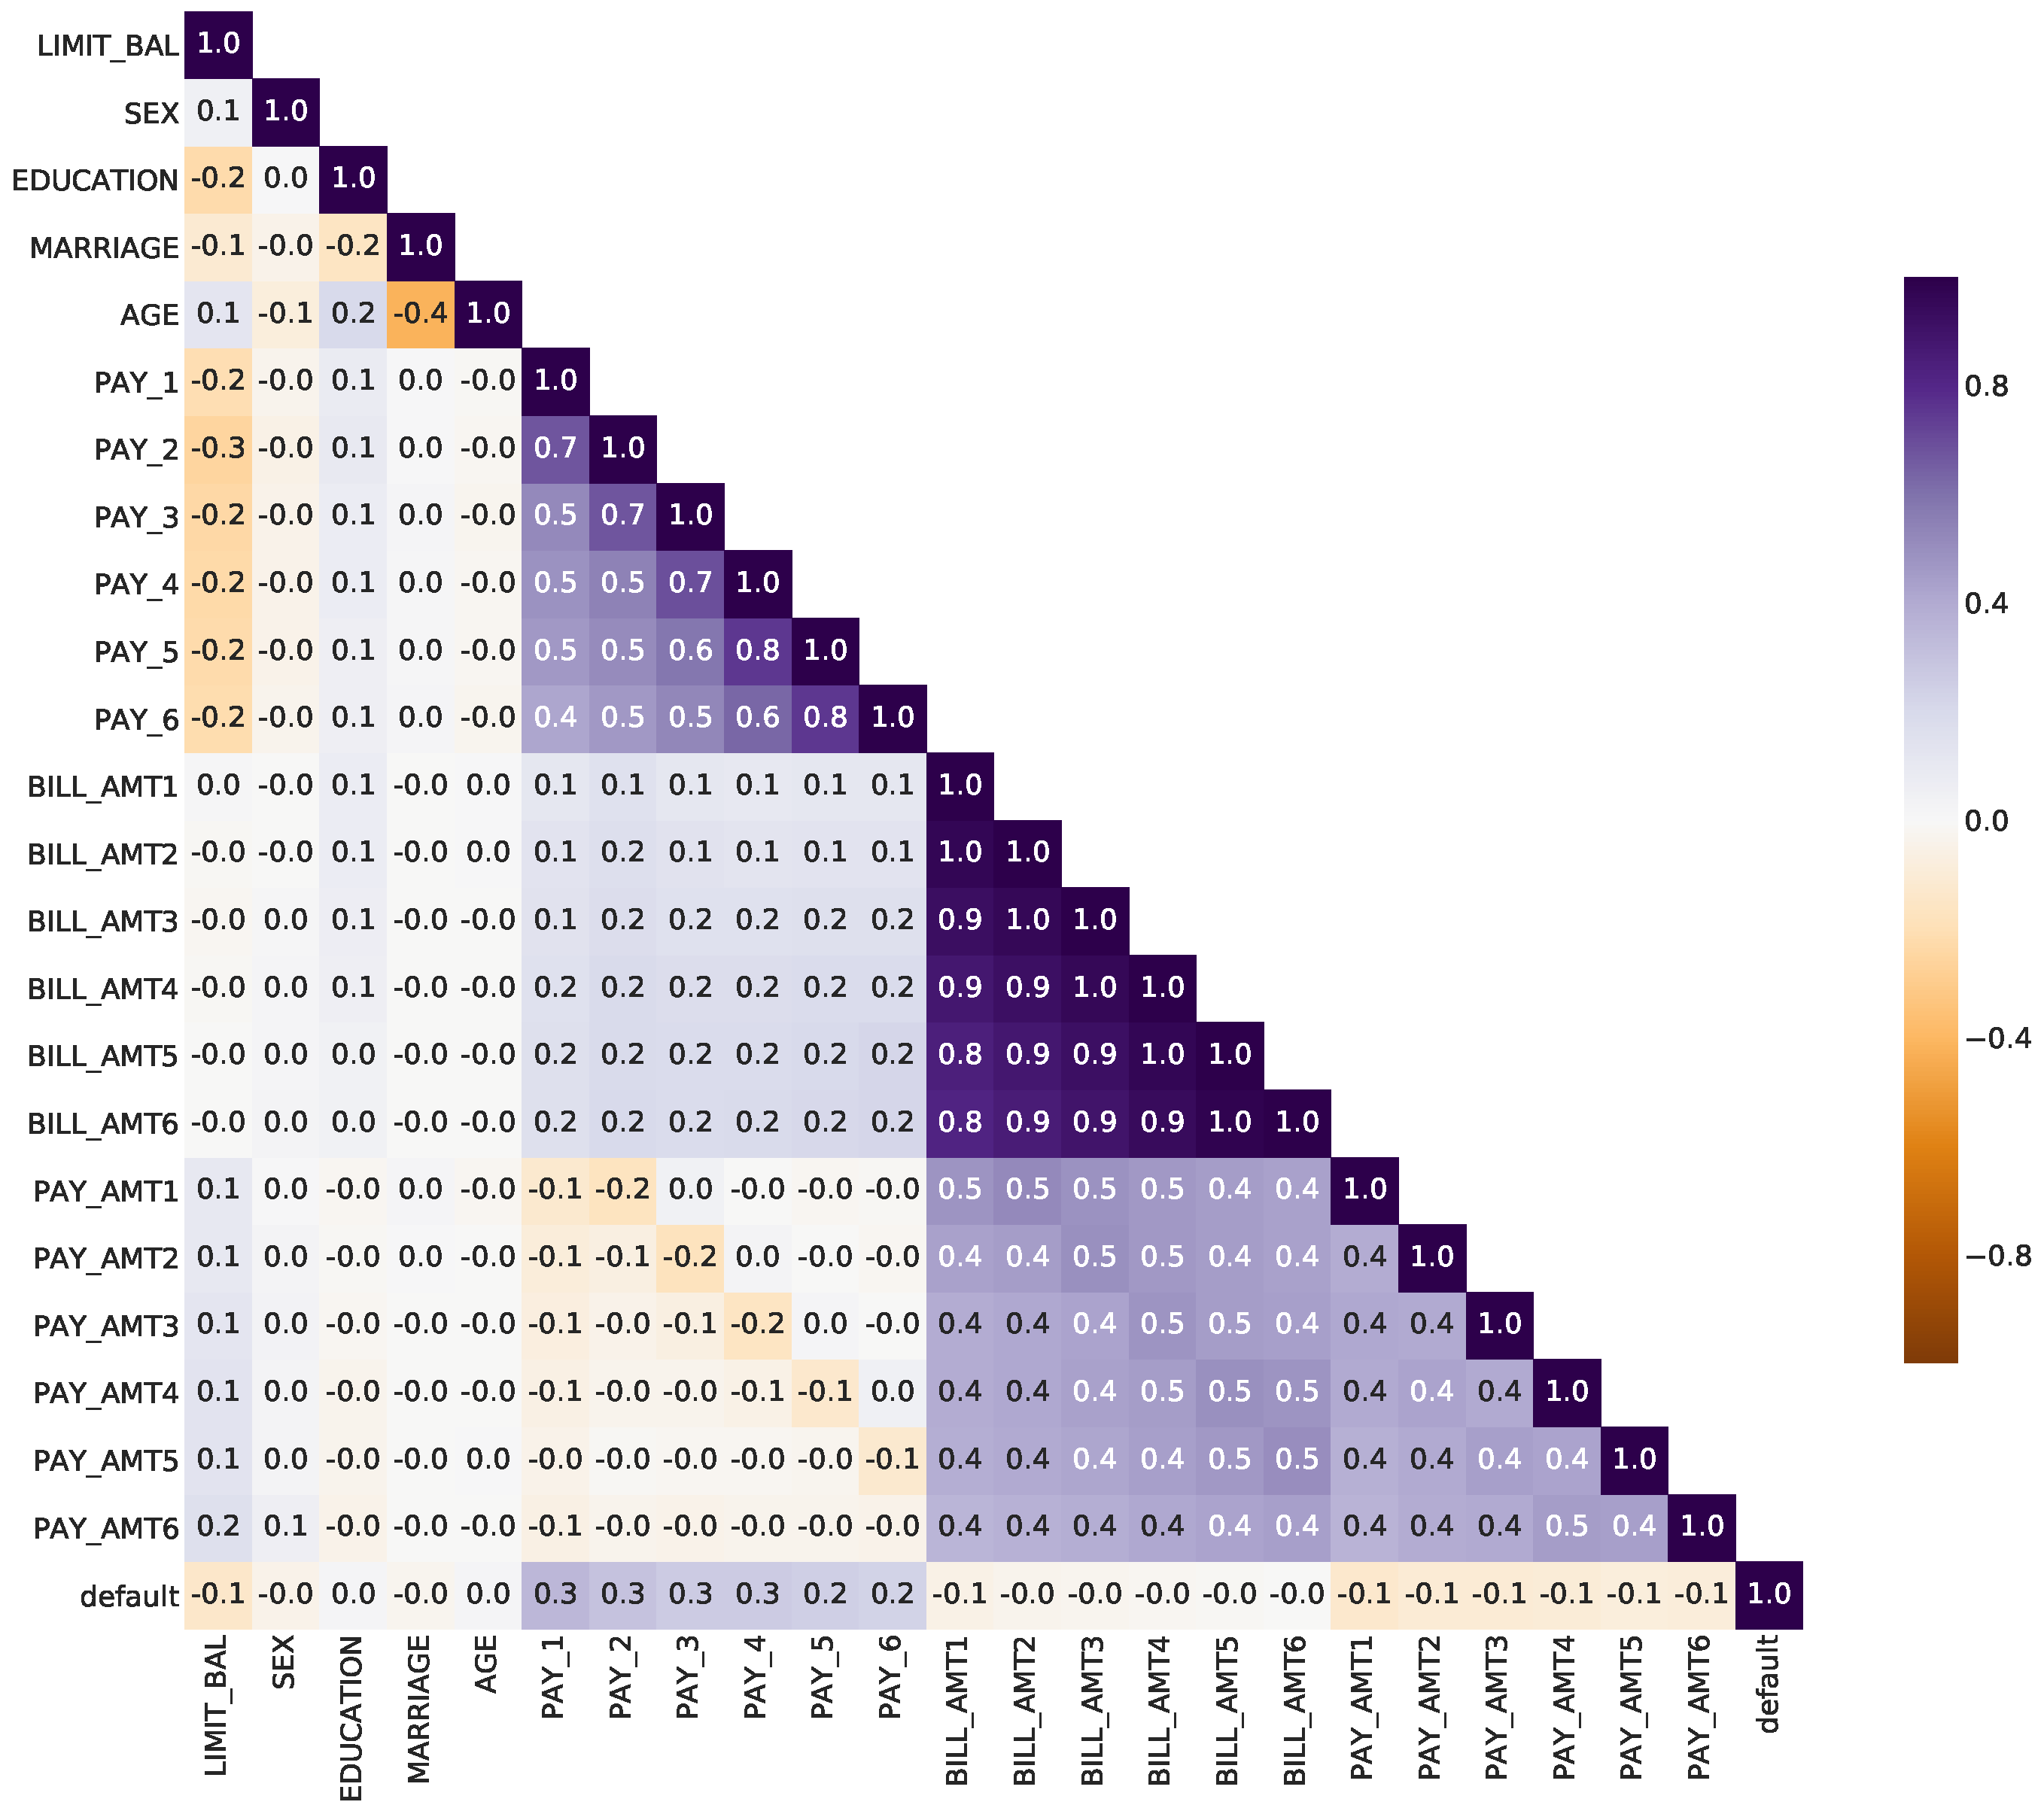
\includegraphics[scale=0.4]{../figs/CC_corr_all.pdf}
    \caption{Correlation matrix between all the 24 columns of the credit card classification dataset.}
    \label{fig:CC_corr_all}
\end{figure}

\end{appendices}
\end{document}
